\documentclass[aip,cha,reprint,amsmath,amssymb,longbibliography]{revtex4-2}
\usepackage{graphicx}
\usepackage{seqsplit}

\newcommand{\sci}[2]{\ensuremath{#1\times10^{#2}}}
\newcommand{\tenp}[1]{\ensuremath{10^{#1}}}
\newcommand{\lam}[1]{\ensuremath{\lambda_{\mathrm{#1}}}}
\newcommand{\lref}{\ensuremath{\lambda_{\mathrm{ref}}}}
\newcommand{\nH}{\ensuremath{n_{\mathrm{H2}}}}
\newcommand{\nconv}{\ensuremath{n_{\mathrm{conv}}}}
\newcommand{\Ech}{\ensuremath{E_{\mathrm{ch}}}}
\newcommand{\Kc}{\ensuremath{K_{\mathrm{c}}}}
\newcommand{\Sec}[1]{Sec.~\ref{#1}}
\newcommand{\hash}[1]{\texttt{\seqsplit{#1}}}

\begin{document}

\title{Largest Lyapunov exponent estimators on the standard map: a preregistered numerical study}

\author{georgehadji}
\affiliation{Independent researcher}

\begin{abstract}
We report a preregistered numerical study of largest-Lyapunov-exponent estimators on the standard map.
The scope is one panel from a single draw (a single seed), run in Float64, with five nonzero kick values and one start per kick value in the reproduction test (H4).
The panel had 883 orbits, including 13 exact-exponent controls.
The claim of asymptotic equivalence (H1) was falsified.
The failure is carried by sub-rule H1c alone, with 162 of 209 eligible orbits passing, a pass fraction of 0.775119617225 against a limit of 0.90.
H1 is evaluated in Float64 at the horizon $N_1=$\tenp{7}, and H1c compares L2 run in wrapped coordinates with L5 in lifted coordinates.
The claim of finite-time inequivalence (H2) was not supported (NEGATIVE).
Over the 355 orbits of the preregistered set $W$ the median of $R(\nH)$ was \sci{2.23588035691}{-5} against a threshold of 0.10.
The regime dependence of the convergence time (H3) was supported, with a ratio of medians of 11213.7767857.
The reproduction of the reference values of Sala and Artuso (H4) did not reproduce at $K=\pi/2$, where we obtained 0.256066843848 against 0.298.
It passed at $K=2\pi$, where we obtained 1.17018723872 against 1.172.
The label rule H5 was supported under its three sub-rules (H5a, H5b, H5c).
The ladder test forced 35 of the 92 ladder-subset labels to unresolved (exploratory item E3).
Cost and sensitivity are reported without a decision rule.
The code is released as Chaoslab v0.1.1 (TOOL), a tagged and documented release with the same computing code.
\end{abstract}

\maketitle

\begin{quotation}
Many methods exist to measure how fast nearby orbits of a chaotic system separate.
The rate is called the largest Lyapunov exponent.
This study compares several such methods on the standard map, a simple model of chaotic motion.
We tested two claims.
The first is that the methods agree after a long run.
The second is that they differ over short, realistic runs.
The rules for deciding each claim were written down and frozen before any data existed.
This is called preregistration.
It prevents the analyst from choosing the test after seeing the result.
The first claim was falsified, because one comparison fell below its limit.
That comparison is between the two-trajectory method and the Householder QR method, the default reference.
The second claim has two tests with different verdicts.
The relative spread among methods at short times was far below its preregistered level.
The convergence time was longer over the preregistered weak-chaos set than over the strong-chaos set.
One of two published reference values did not reproduce, and the other did.
The results come from one panel of orbits, one random draw and double precision.
\end{quotation}

\section{Introduction}
\label{sec:intro}

This paper reports a preregistered numerical study of largest-Lyapunov-exponent estimators on the standard map.
The study tests two claims of the project, C1 (asymptotic equivalence) and C2 (finite-time inequivalence).
The claim texts below are quoted from the project statement of research questions.
They are claims of the study.
They are not statements supported by the literature cited in this paper.

Claim C1, as stated in the project statement: ``Benettin, QR (Gram-Schmidt / Householder), stabilized SVD and well-conditioned tangent-map methods agree on $\lambda_1$ when run long enough at adequate precision.''

Claim C2, as stated in the project statement: ``Finite-time LE estimators differ substantially over realistic budgets, most of all in weak chaos, sticky layers and near separatrices.''
Here LE stands for Lyapunov exponent and $\lambda_1$ for the largest exponent.
The tests of C2 in this study run over the preregistered set $W$ of \Sec{sub:notation}, whose composition is shown in Tables~\ref{tab:h2cell} and~\ref{tab:h3cell}.

The study also attempts to reproduce two published values.
Sala and Artuso give 0.298 at $K=\pi/2$ and 1.172 at $K=2\pi$ \cite{SalaArtuso2015}.

Two published comparators serve for the chaotic-sea exponent.
These are the fit of Shevchenko \cite{Shevchenko2014} and the line $\ln(K/2)$ of Chirikov \cite{Chirikov1979}.
The study uses both as comparators that never pass or fail.

Lyapunov spectra are usually computed by renormalising tangent vectors and orthogonalising them by Gram-Schmidt \cite{Benettin1980a,Benettin1980b,ShimadaNagashima1979}.
Gram-Schmidt, Householder and continuous QR variants were compared on a Toda chain; the discrete variants differed by much less than the fluctuations of the finite-time values, and continuous QR took about 40 times the CPU time of Gram-Schmidt \cite{Geist1990}.
Singular-value methods take the singular values of a product of Jacobians without forming the product \cite{Stewart1997}, and their theory holds for systems with stable and distinct exponents \cite{DieciElia2006}.

Finite-time effects are known in particular settings.
For standard-like maps the finite-time exponent carries an initial-vector transient that fades like $1/n$ \cite{SalaArtuso2015}.
For the two-trajectory method on flows, the renormalisation time and the initial distance can produce a spurious largest exponent \cite{DubeibeBermudezAlmanza2014}.
Sticky orbits need long runs: a finite-time exponent in an extreme sticky zone of the standard map had not converged after $5\times10^{7}$ iterations, against about \tenp{7} in the chaotic sea \cite{HarsoulaKaramanosContopoulos2019}, and one orbit at $k=0.975$ looks confined for \tenp{6} steps and escapes after $2.3\times10^{9}$ \cite{Meiss2015}.
Round-off induced divergence of orbits has been related to the reversibility error in discrete-time systems \cite{FarandaMestreTurchetti2012}.
This study compares the estimators above on one map, over five orbit regimes, with a precision ladder on a subset of the orbits.

This paper reports the study as preregistered.
It adds no new claim, softens no result and offers no reinterpretation.
\Sec{sec:methods} gives the design, the notation and the run identity.
\Sec{sec:h1} to \Sec{sec:h5} give the confirmatory results for hypotheses H1 to H5.
Exploratory subsections inside those sections are marked EXPLORATORY: E1 and E2 in \Sec{sub:h1exp}, E4 in \Sec{sub:h4exp}, and E3 and E5 in \Sec{sub:h5exp}.
\Sec{sec:cost} gives cost and sensitivity.
\Sec{sec:expl} gives the exploratory items E6 and E7.
\Sec{sec:lim} and \Sec{sec:concl} give the limitations and the conclusion.
The Data availability section follows the conclusion.

\section{Methods and preregistration}
\label{sec:methods}

\subsection{Preregistration}
\label{sub:prereg}

The decision rules were frozen on 2026-10-17, before any data existed.
Amendments A1 to A6 were all frozen before the first study data file.
The rules are applied as frozen, with the deviations listed in \Sec{sub:dev}.
The analysis output also lists 14 readings where the frozen text is silent (\Sec{sub:dev}).
Amendments A1 to A4 are described briefly.
A1 sets the hash rule, the T predicate, the screening direction, the windowed estimate, the Newton periodic-point search, the subset caps and the machine-readable panel inputs.
A2 handles a ghost pair of periodic points at $K=2\pi$ and is superseded by A3.
A3 sets the acceptance test of the periodic-point search.
A4 adds the machine-readable run block, the setup check, the cost cap and pilot, the backend agreement and the scope of the control bound.
The content of A5 and A6 is given in \Sec{sub:dev}.

The preregistered value types were FALSIFIES (C1, C2), REPRODUCES \cite{SalaArtuso2015}, TOOL and NEGATIVE allowed.
Claim C3 is out of scope.

TOOL claim: the library Chaoslab, release v0.1.1.
Every method the run used has catalog status \texttt{verified}, as stated in the preregistration.
Release v0.1.1 is tagged and carries user documentation, and its package code differs from the analysis commit only in docstrings and in a file-descriptor conversion that is a no-op on Julia 1.13.2, the Julia version of the run (see Data availability).

The preregistration header is identified by the SHA-256 value in Table~\ref{tab:run}.
The location of the frozen text is given in the Data availability section.

\subsection{Notation and definitions}
\label{sub:notation}

This subsection restates the notation of the study design.
The standard map is iterated in lifted coordinates,
\begin{equation}
p_{n+1}=p_n+K\sin x_n,\qquad x_{n+1}=x_n+p_{n+1},
\label{eq:map}
\end{equation}
with the tangent map
\begin{equation}
DT_K(x_n,p_n)=\begin{pmatrix}1+K\cos x_n & 1\\ K\cos x_n & 1\end{pmatrix},\qquad \det DT_K=1 .
\label{eq:tangent}
\end{equation}
The map is symplectic, so the two exponents of an orbit are $\{\lambda,-\lambda\}$.

\begin{itemize}
\item \emph{Variables and horizons.}
The map variables are $(x,p)$.
The H4 start is $x_0=$\tenp{-3} and $p_0=-$\tenp{-3}.
$K$ is the kick parameter.
The horizons are $N_1=$\tenp{7} (all orbits), $N_{\mathrm{long}}=$\tenp{8} (designated subset) and $N_B=$\tenp{6} (precision ladder).
$N$ is the horizon of the series used; $R(n)$ and \nconv\ use the horizon-$N_1$ series of every orbit.

\item \emph{Finite-time exponent.}
$\lambda_m(n)$ is the finite-time largest Lyapunov exponent of method $m$ after $n$ map steps, in natural log per step, with the Euclidean 2-norm on the lifted $(x,p)$ tangent vector.
L9 uses the largest finite-time singular value of the product.
$\lref$ of an orbit is $\lam{L5}$ at the longest Float64 horizon of that orbit.

\item \emph{Methods.}
L1 is Benettin.
L2 is the two-trajectory method, an approximation of the largest exponent.
L3 is CGS, L4 is MGS, L4b is RGS, L5 is Householder (the default reference), L5b is the H2 diagonal iteration path, L6 is Givens, and L9 is the stabilized SVD ($d=2$).
Their algorithm details are in the preregistration and the repository, not here.

\item \emph{Method sets.}
$Q=\{\mathrm{L3},\mathrm{L4},\mathrm{L4b},\mathrm{L5},\mathrm{L5b},\mathrm{L6}\}$.
The variational set is $V=\{\mathrm{L1}\}\cup Q\cup\{\mathrm{L9}\}$.
The expression $\{\mathrm{L1}\}\cup Q$ means L1 together with the members of $Q$.

\item \emph{Parameters.}
$\tau$ is the fixed reorthonormalization interval of the $Q$ methods (primary $\tau=1$).
$\epsilon$ is the perturbation size of L2 (primary $\epsilon_0=$\tenp{-8}).
The primary initial deviation direction is the angle $\pi/4$ from the $x$ axis.
On the designated subset four more ``direction offsets'' are used: 0.3, $0.3+\pi/5$, $0.3+2\pi/5$ and $0.3+3\pi/5$.
The precisions are Float64, Double64 and BigFloat.

\item \emph{Spreads and ratios.}
The spreads and the ratio are
\begin{align}
\Delta_{QB}(n) &= \max_{m\in\{\mathrm{L1}\}\cup Q}\lambda_m(n)-\min_{m\in\{\mathrm{L1}\}\cup Q}\lambda_m(n),\\
\Delta_V(n) &= \max_{m\in V}\lambda_m(n)-\min_{m\in V}\lambda_m(n),\\
R(n) &= \Delta_V(n)/\lref \qquad \text{(H2)}.
\end{align}
The convergence time \nconv\ is defined in the rule for H3 (\Sec{sub:h3rule}); the series are stored at recorded values of $n$, so \nconv\ takes recorded values of $n$.

\item \emph{Design classes.}
T (KAM torus), R (resonant), C (chaotic sea), S (sticky) and X (near a separatrix or a hyperbolic fixed point).
Design class is the a-priori intended class of an orbit.
A cell is a $K$ value times a design class.

\item \emph{Controls.}
The controls are the exact periodic points of the map and one hyperbolic linear map, whose exponents are known analytically.
``Info'' controls are defined in \Sec{sub:dev}.

\item \emph{Sets.}
$\Ech$ is the set of design class C orbits at $K>0$ plus the controls with positive analytic exponent (H1).
The weak-chaos set $W$ is defined below.
The strong-chaos set $S$ is the class C orbits at $K=2\pi$ and $K=10$ (H3).
$S_D$ is the designated subset and $S_L$ is the ladder subset, nested in the panel; $S_L$ carries the Double64 and BigFloat runs.
The symbol $S$ names three things in this paper: the panel class S (sticky), the strong-chaos set $S$ of H3 and, as $S_L$, the ladder subset.
The context says which.

\item \emph{Definition of $W$ (preregistered).}
$W$ = orbits with instability label ``positive growth supported'' in the design classes sticky or near-separatrix at any $K>0$, plus chaotic-sea orbits at $K\le\Kc$.
The name ``weak-chaos set'' is the preregistration's.
By this definition $W$ contains class S and class X orbits at the large $K$ values as well, and Tables~\ref{tab:h2cell} and~\ref{tab:h3cell} show its cells.
The name does not mean that every member of $W$ is in weak chaos.

\item \emph{Labels.}
Each orbit carries two labels.
The instability label takes the values ``positive growth supported'', ``none detected on the tested horizon'' and ``unresolved''.
The structure label takes the values ``periodic'', ``quasiperiodic'', ``irregular'' and ``unresolved''.
Four disagreement tests force a label to ``unresolved'': the precision ladder test (on $S_L$ only), the estimators test (any failure of H1a or H1b on that orbit), the direction test (on the designated subset only) and the diagnostics test (a pairing, determinant or orthogonality residual above its tolerance for L5).
A label is ``forced'' when one of these tests sets it to ``unresolved''.
The thresholds of the label rules are in the preregistration.

\item \emph{Drift and kept orbits.}
An orbit is flagged ``drift'' when its lifted $|p|$ exceeds \tenp{6} at any recorded time.
Drift orbits are removed from $\Ech$, $W$ and $S$.
``Kept'' orbits are the orbits not dropped as drift or excluded.

\item \emph{Bootstrap.}
The bootstrap intervals are percentile intervals at the 95 percent level with $10^{4}$ resamples.
Orbits are resampled with replacement, and $W$ and $S$ are resampled independently.
\end{itemize}

\subsection{Panel and sets}
\label{sub:panel}

The study compares estimators on a panel of 883 orbits.
The panel has the following cells.
There are 13 controls in the cell of $K$ index 0, and 40 orbits each in classes R and T at $K$ index 1.
At $K$ index 2 the classes are C, R, S, T and X with 40, 40, 25, 40 and 40 orbits.
At $K$ index 3 and 4 the classes are C, R, S, T and X with 40 orbits each.
At $K$ index 5 the classes are C, S, T and X with 40, 5, 40 and 40 orbits.
At $K$ index 6 the classes are C and X with 40 orbits each.
Cells that are short, empty or undefined are listed in item E6 (\Sec{sec:expl}).

$K$ index 0 holds the exact-exponent controls.
$K$ index 1 is $K=0$.
$K$ index 2 to 6 are $K=0.5$, 0.971635406 ($\Kc$, the breakup value of the golden-mean KAM torus, as given in \cite{FrahmShepelyansky2010,CarlettiLaskar2000} and fixed in the preregistration), 1.57079632679 ($\pi/2$), 6.28318530718 ($2\pi$) and 10.

``Class S'' is a panel class.
It is not the ``strong-chaos set $S$'' of H3, which is the class C orbits at $K=2\pi$ and $K=10$.

One orbit, orbit 881, is dropped as drift.
Under the preregistration, drift orbits are removed from $\Ech$, $W$ and $S$.
H5b is defined on all panel orbits and uses 883.
The sets used by the decision rules have these sizes: $\Ech$ 209, $W$ 355, $S$ 80 and $S_L$ 92.
H5b uses 883 orbits and H5c uses 334.

The analysis code reads $S$ as the class C orbits at $K=2\pi$ and $K=10$ without a label condition.
It reads $\Ech$ as class C at $K>0$ (plus the controls, \Sec{sub:h1rule}).
For $W$ this paper uses the preregistered definition of \Sec{sub:notation}.
The analysis code reports a shorter phrase for $W$ in its list of readings, class C at $0<K\le\Kc$.
That phrase is not the frozen definition and does not describe the cells of Tables~\ref{tab:h2cell} and~\ref{tab:h3cell}, which also contain classes S and X (limitation~6, \Sec{sec:lim}).

The estimator methods L1 to L9 and $Q$ are defined in \Sec{sub:notation}.
The repository holds the details.

\subsection{Run identity}
\label{sub:run}

All reported numbers come from one fully automatic analysis run over the stored series.
The run completed with 1363 chunks, all with status ok.
Table~\ref{tab:run} identifies the run.

\begin{table*}
\caption{Run identity.}
\label{tab:run}
\footnotesize
\begin{ruledtabular}
\begin{tabular}{ll}
Item & Value \\
\hline
Analysis commit (git) & \hash{d31b655d0c33e2f2f1a67bbbdeba9c8c8a3fd036} \\
Run commit (git, recorded by the run manifest) & \hash{3e405f3324f8d25162580d3380db26c877d7ca63} \\
Package version & 0.0.1 \\
Panel SHA-256 & \hash{881874d26aa8883caa0545331ba167a3f2c9e3c249cdb6ba32ad39c98ad348d5} \\
Preregistration header SHA-256 & \hash{62011ba5af514da4f1238aef9ae6cb35ca21093c4343b71dd696df360b9994bf} \\
Manifest SHA-256 & \hash{ae6ec80eb08fbd6e98aeef1fbf840a567a03102ab943f2ae0aaf2b3e367f191d} \\
Parameter file SHA-256 & \hash{a544130bc56dc66d8b1f7ec5d1e54197306f14dc19c7cd22fdbd94e4534b7282} \\
Bootstrap seed & 20261012 \\
Run status & complete, 1363 chunks, all with status ok \\
\end{tabular}
\end{ruledtabular}
\end{table*}

The first git commit in Table~\ref{tab:run} is that of the analysis code, which produced the tables and figures.
The run manifest records the second.
The run commit is an ancestor of the analysis commit, and between them only the analysis code, its figure extension, the command-line entry point and the project file change.
The stored series therefore come from the run commit and the tables and figures from the analysis commit, with the same series code at both (limitation~8, \Sec{sec:lim}).

\subsection{Deviations from the frozen text and readings}
\label{sub:dev}

The frozen text was applied with the deviations that the analysis code states.

\begin{enumerate}
\item L2 runs in wrapped coordinates (Amendment A5 item 1).
H1c compares the wrapped L2 value with the lifted L5 value of the same orbit.
\item The $\tau$ sweep records an orthonormalisation breakdown as a result, not as a failure (A5 item 2).
\item The control bound applies to controls 871, 873, 875, 877, 879 and 883 (A5 item 3).
Controls 878, 880, 881 and 882 are reported as info and are not held to the bound.
\item The control bound of L9 is \sci{5.0}{-8} and that of the other methods is \sci{1.0}{-8} (A6).
\item The run manifest records no overrides.
\end{enumerate}

The analysis output lists 14 readings where the frozen text is silent.
Two bear directly on the verdicts.
The first is that H5a is read from the per-precision labels before the ladder test acts, and H5 is supported only if H5a, H5b and H5c all pass.
The second is the definitions of $S$, $W$ and $\Ech$ as the analysis code reads them (\Sec{sub:panel}).
The other twelve readings are not described in this paper.

\section{Results for H1 (claim C1): FALSIFIED}
\label{sec:h1}

\subsection{Preregistered rule}
\label{sub:h1rule}

The rule applies on $\Ech$, which is class C orbits at $K>0$ plus the exact-exponent controls.
The horizon is $N_1=$\tenp{7}.
An orbit passes H1a if the spread over $\{\mathrm{L1}\}\cup Q$ is at most \tenp{-8}.
It passes H1b if $|\lam{L9}-\lam{L5}|$ is at most \tenp{-6}.
It passes H1c if $|\lam{L2}-\lam{L5}|$ is at most \sci{5}{-3} at $\epsilon_0=$\tenp{-8}.

H1 is SUPPORTED only if the pass fraction is at least 0.98 for H1a and H1b and at least 0.90 for H1c.
It is FALSIFIED if any sub-rule is below its limit.

\subsection{Measured}
\label{sub:h1meas}

There were 209 eligible orbits.
The analysis code reports the verdict falsified.
Table~\ref{tab:h1} gives the three sub-rules.

\begin{table}
\caption{H1 sub-rules on $\Ech$.}
\label{tab:h1}
\begin{ruledtabular}
\begin{tabular}{lcccc}
Sub-rule & Limit & Passing orbits & Fraction & Result \\
\hline
H1a & 0.98 & 209 of 209 & 1.0 & pass \\
H1b & 0.98 & 209 of 209 & 1.0 & pass \\
H1c & 0.90 & 162 of 209 & 0.775119617225 & fail \\
\end{tabular}
\end{ruledtabular}
\end{table}

H1 is falsified.
The H1c pass fraction was 162 of 209, which is 0.775119617225, against the limit of 0.90.
The shortfall is carried by sub-rule H1c alone.
H1a and H1b were met in full.

Table~\ref{tab:h1cell} gives H1c by cell.

\begin{table}
\caption{H1c passing orbits by cell.}
\label{tab:h1cell}
\begin{ruledtabular}
\begin{tabular}{lcc}
Cell & Orbits & H1c pass \\
\hline
controls & 9 & 9 \\
$K$ index 2 & 40 & 27 \\
$K$ index 3 & 40 & 13 \\
$K$ index 4 & 40 & 33 \\
$K$ index 5 & 40 & 40 \\
$K$ index 6 & 40 & 40 \\
\end{tabular}
\end{ruledtabular}
\end{table}

The 47 failing orbits sit in three $K$ cells.
At $K$ index 2, 27 of 40 orbits pass.
At $K$ index 3, 13 of 40 pass.
At $K$ index 4, 33 of 40 pass.
$K$ index 5 and 6 pass 40 of 40, and the 9 controls pass.
H1a and H1b pass in every cell.
Every failing orbit has $|\lam{L2}-\lam{L5}|$ above 0.005.
The smallest is 0.00548462883667 and the largest is 0.0353748064771.
On the failing orbits the largest $\Delta_{QB}$ is \sci{9.66310365058}{-14} and the largest $|\lam{L9}-\lam{L5}|$ is \sci{3.58331395889}{-7}.
None of them breaks H1a or H1b.
Figures~\ref{fig:F1} and~\ref{fig:F1b} show the $\lambda_m(n)$ curves.

\begin{figure*}
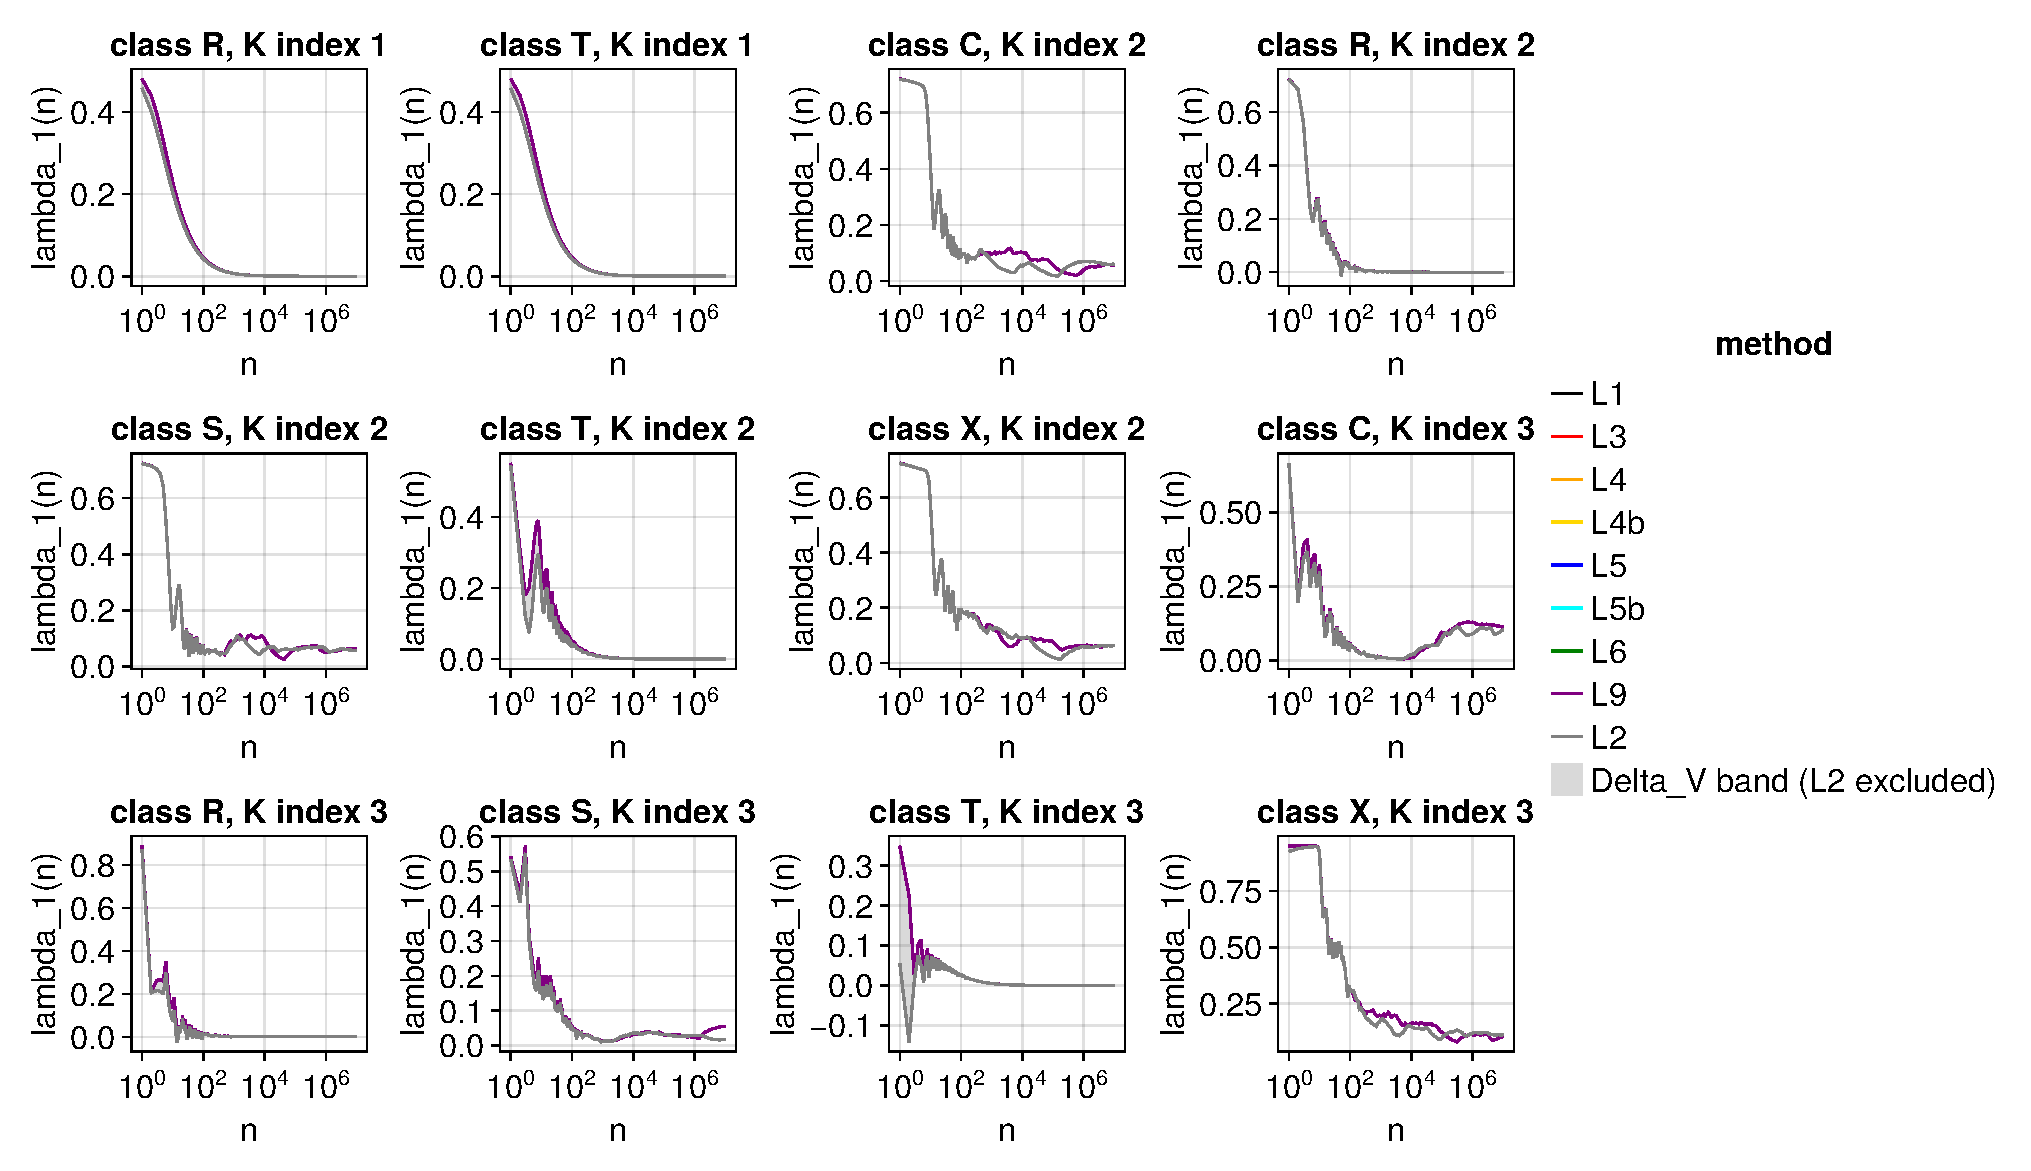
\includegraphics[width=\textwidth]{../figures/p1-le-benchmark-fig-F1a.pdf}
\caption{Finite-time exponent $\lambda_1(n)$ of the nine methods for the first drawn orbit of each populated cell (design class and $K$ index), $K$ index 1 to 3, with the band between the smallest and the largest of the eight methods of $V$ (L2 excluded).}
\label{fig:F1}
\end{figure*}

\begin{figure*}
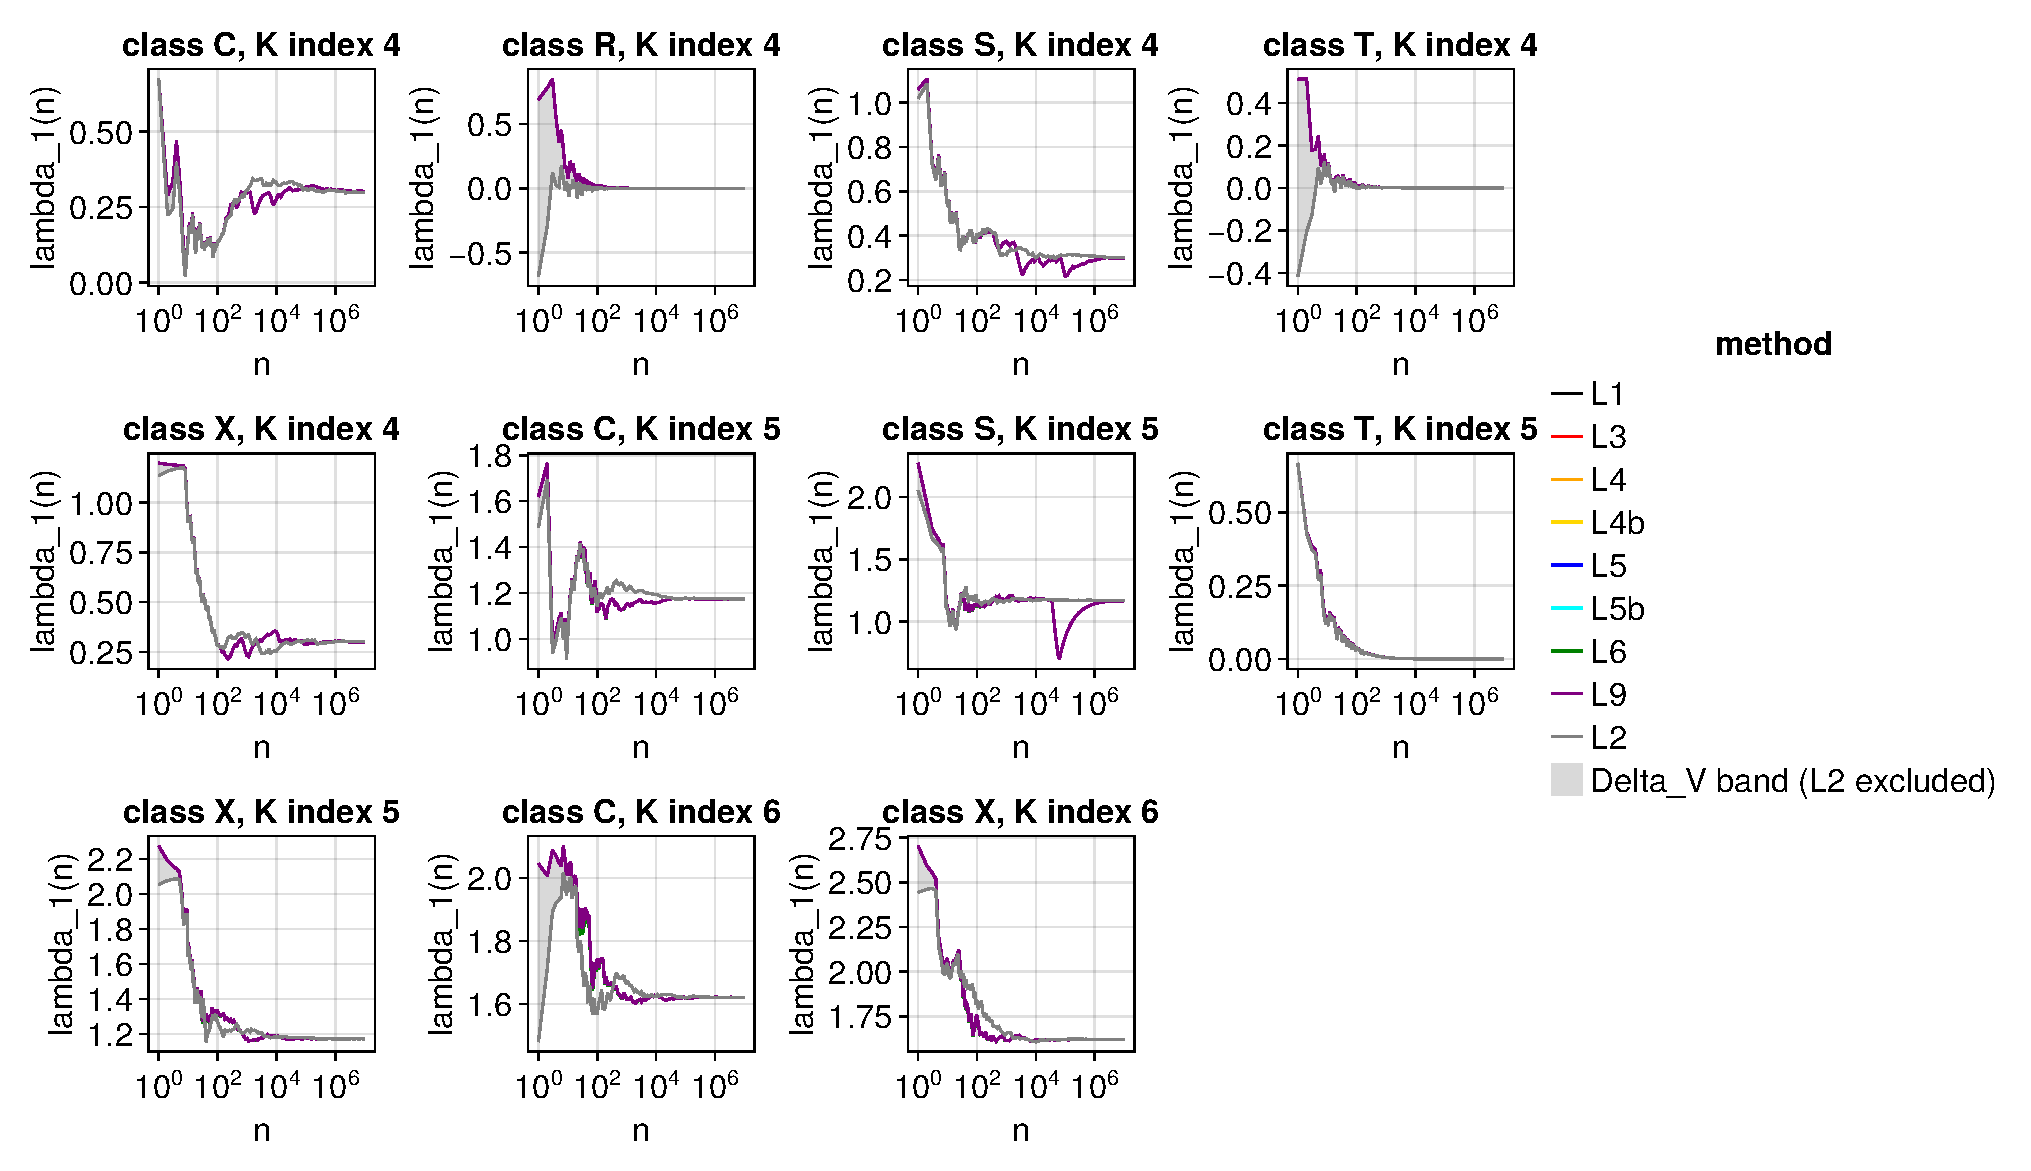
\includegraphics[width=\textwidth]{../figures/p1-le-benchmark-fig-F1b.pdf}
\caption{As Fig.~\ref{fig:F1}, for $K$ index 4 to 6.}
\label{fig:F1b}
\end{figure*}

\subsection{Exact-exponent controls}
\label{sub:ctrl}

The controls under the bound are 871, 873, 875, 877, 879 and 883.
Table~\ref{tab:ctrl} gives the largest deviation over the methods.

\begin{table}
\caption{Exact-exponent controls under the bound.}
\label{tab:ctrl}
\begin{ruledtabular}
\begin{tabular}{lcc}
Control & Largest deviation & L9 deviation \\
\hline
871 & \sci{5.26802590439}{-9} & \sci{5.26802579337}{-9} \\
873 & \sci{2.48736364838}{-9} & \sci{8.326783706990001}{-12} \\
875 & \sci{5.16177345311}{-9} & \sci{1.82781789704}{-9} \\
877 & \sci{1.79536172595}{-8} & \sci{1.79536172595}{-8} \\
879 & \sci{2.28260139679}{-8} & \sci{2.28260139679}{-8} \\
883 & \sci{1.11022302463}{-16} & \sci{1.11022302463}{-16} \\
\end{tabular}
\end{ruledtabular}
\end{table}

The largest deviations lie within the bounds of Amendment A6.
For controls 877 and 879 the largest deviation is the L9 deviation.
It is above \tenp{-8} and below the L9 control bound of \sci{5.0}{-8}.
The table does not give the other methods' deviations on these two controls separately.

Accounting for the control ids.
The panel counts 13 controls in the cell of $K$ index 0, and Table~\ref{tab:h1cell} counts 9 controls in $\Ech$.
The list of controls with positive analytic exponent has 10 ids: the six of Table~\ref{tab:ctrl} and the four info controls 878, 880, 881 and 882 (item E2).
The other 3 controls, orbits 872, 874 and 876, start at the elliptic fixed point $(\pi,0)$ at $K=0.5$, $\Kc$ and $\pi/2$ and have analytic exponent 0.
$\Ech$ and that list take only controls with positive analytic exponent, so these three appear in neither; they serve the setup check of the Double64 and BigFloat runs and enter H5b with every panel orbit.
Orbit 881 is an info control and is the orbit dropped as drift (\Sec{sub:panel}).

\subsection{Reading}
\label{sub:h1read}

The preregistered rule for C1 is not met.
H1 is reported as falsified.
The falsification rests on sub-rule H1c alone.
It was evaluated in Float64 at $N_1=$\tenp{7} on one panel, and H1c compares L2 in wrapped coordinates with L5 in lifted coordinates (\Sec{sub:dev}, item 1; limitation~4 in \Sec{sec:lim}).
The analysis does not show whether the coordinate choice accounts for any part of the H1c result.

\subsection{Exploratory items E1 and E2 (EXPLORATORY)}
\label{sub:h1exp}

Everything in this subsection is EXPLORATORY.
No frozen rule applies and no cause is claimed.

E1 (EXPLORATORY): where the H1c failures sit.
The 47 H1c failures are in three $K$ cells.
$K$ index 2 has 13 of 40 failing (27 pass).
$K$ index 3 has 27 of 40 (13 pass).
$K$ index 4 has 7 of 40 (33 pass).
$K$ index 5 and 6 have no failures (40 of 40 pass each) and the 9 controls all pass.
The failing ids fall in three ranges: 13 ids between 166 and 196, 27 between 346 and 385, and 7 between 549 and 580.
These counts match the per-cell failure counts, but the analysis does not state the orbit-to-cell mapping.
The analysis does not show why the failures sit at the three smaller $K$.

E2 (EXPLORATORY): the info controls.
Controls 878, 880, 881 and 882 are reported as info.
Their largest deviations are 0.222903869545, 0.443364672685, 0.650205817015 and 0.103506221066.
These are far above the bound that applies to the other six controls.
Amendment A5 item 3 designates these four as the controls reported as info; the analysis output describes them as the controls whose binary64 start is not an exact periodic point.
That description is not tested here.
The analysis does not say more.

\section{Results for H2 (claim C2): NOT SUPPORTED (NEGATIVE)}
\label{sec:h2}

\subsection{Preregistered rule}

$R(\nH)=\Delta_V(\nH)/\lref$ is evaluated at $\nH=$\tenp{4} steps over the set $W$ defined in \Sec{sub:notation}.
The preregistration names $W$ the weak-chaos set.
$W$ = orbits with instability label ``positive growth supported'' in the design classes sticky or near-separatrix at any $K>0$, plus chaotic-sea orbits at $K\le\Kc$.

H2 is SUPPORTED if the median of $R(\nH)$ is at least 0.10 and the lower end of its 95 percent bootstrap interval ($10^{4}$ resamples of orbits) is at least 0.05.
Otherwise the null is reported.

\subsection{Measured}

$W$ has 355 orbits.
The median of $R(\nH)$ is \sci{2.23588035691}{-5}.
The 95 percent bootstrap interval is [\sci{1.9257235885}{-5}, \sci{2.31226443693}{-5}].
The analysis code reports the verdict not supported.
Both conditions fail.
The median is below 0.10 and the lower end is below 0.05.

\begin{table*}
\caption{H2 against the preregistered thresholds.}
\label{tab:h2}
\begin{ruledtabular}
\begin{tabular}{lccc}
Quantity & Measured & Threshold & Result \\
\hline
Median of $R(\nH)$ over $W$ (355 orbits) & \sci{2.23588035691}{-5} & at least 0.10 & fail \\
Lower end of the 95 percent interval & \sci{1.9257235885}{-5} & at least 0.05 & fail \\
\end{tabular}
\end{ruledtabular}
\end{table*}

This is a null (NEGATIVE) result.
It has the same standing as a pass.
In $W$, the relative spread among the methods of $V$ at \tenp{4} steps is far below the preregistered level.
The frozen rule decides on the pooled $W$.
Table~\ref{tab:h2cell} gives the cells of $W$; the cell results are descriptive.
$W$ is composed of class C at $K$ index 2 and 3, class S at $K$ index 2 to 5 and class X at $K$ index 2 to 6.

\begin{table*}
\caption{H2: $R(\nH)$ by cell of $W$ (descriptive).}
\label{tab:h2cell}
\begin{ruledtabular}
\begin{tabular}{llccccl}
Class & $K$ index & $W$ orbits & Median & Lo & Hi & Note \\
\hline
C & 2 & 36 & 0.000685409790935 & \sci{1.21772360607}{-5} & 0.00158551651977 & \\
S & 2 & 21 & \sci{5.42291035617}{-5} & \sci{3.17071908742}{-6} & 0.00145378914565 & \\
X & 2 & 36 & \sci{5.82402750446}{-12} & \sci{7.73045459959}{-13} & \sci{3.49257079589}{-11} & \\
C & 3 & 34 & 0.000380436190835 & \sci{7.27740118397}{-5} & 0.000658941961158 & \\
S & 3 & 37 & 0.000775501992792 & 0.000343310022299 & 0.000939537300147 & \\
X & 3 & 36 & \sci{2.26586896653}{-5} & \sci{2.21983704619}{-5} & \sci{2.30966041916}{-5} & \\
S & 4 & 37 & \sci{9.63721942695}{-5} & \sci{4.60435510795}{-5} & 0.000139046731348 & \\
X & 4 & 37 & \sci{2.32406707119}{-5} & \sci{2.32155590409}{-5} & \sci{2.32870005206}{-5} & \\
S & 5 & 1 & \sci{6.01344714582}{-5} & \sci{6.01344714582}{-5} & \sci{6.01344714582}{-5} & not decidable \\
X & 5 & 40 & \sci{1.92365473742}{-5} & \sci{1.92334364212}{-5} & \sci{1.92413315356}{-5} & \\
X & 6 & 40 & \sci{1.6241799957}{-5} & \sci{1.62397348555}{-5} & \sci{1.62425706568}{-5} & \\
\end{tabular}
\end{ruledtabular}
\end{table*}

No cell median of $R(\nH)$ reaches the threshold of 0.10.
The largest cell median is 0.000775501992792 (class S, $K$ index 3).
The direction of the NEGATIVE verdict therefore holds in every cell as well as in the pooled set.
This is exploratory item E7 (\Sec{sec:expl}) and is not a decision rule.
The cell of class S at $K$ index 5 has 1 orbit, below the minimum set size of 20.
It is not decidable and is neither pass nor fail.
The bootstrap resamples orbits as if they were independent draws (limitation~1, \Sec{sec:lim}).
The cell intervals of Table~\ref{tab:h2cell} are descriptive.
Figures~\ref{fig:F2} and~\ref{fig:F2b} show $R(n)$ by class and $K$, with the pooled series over $W$.

\begin{figure*}
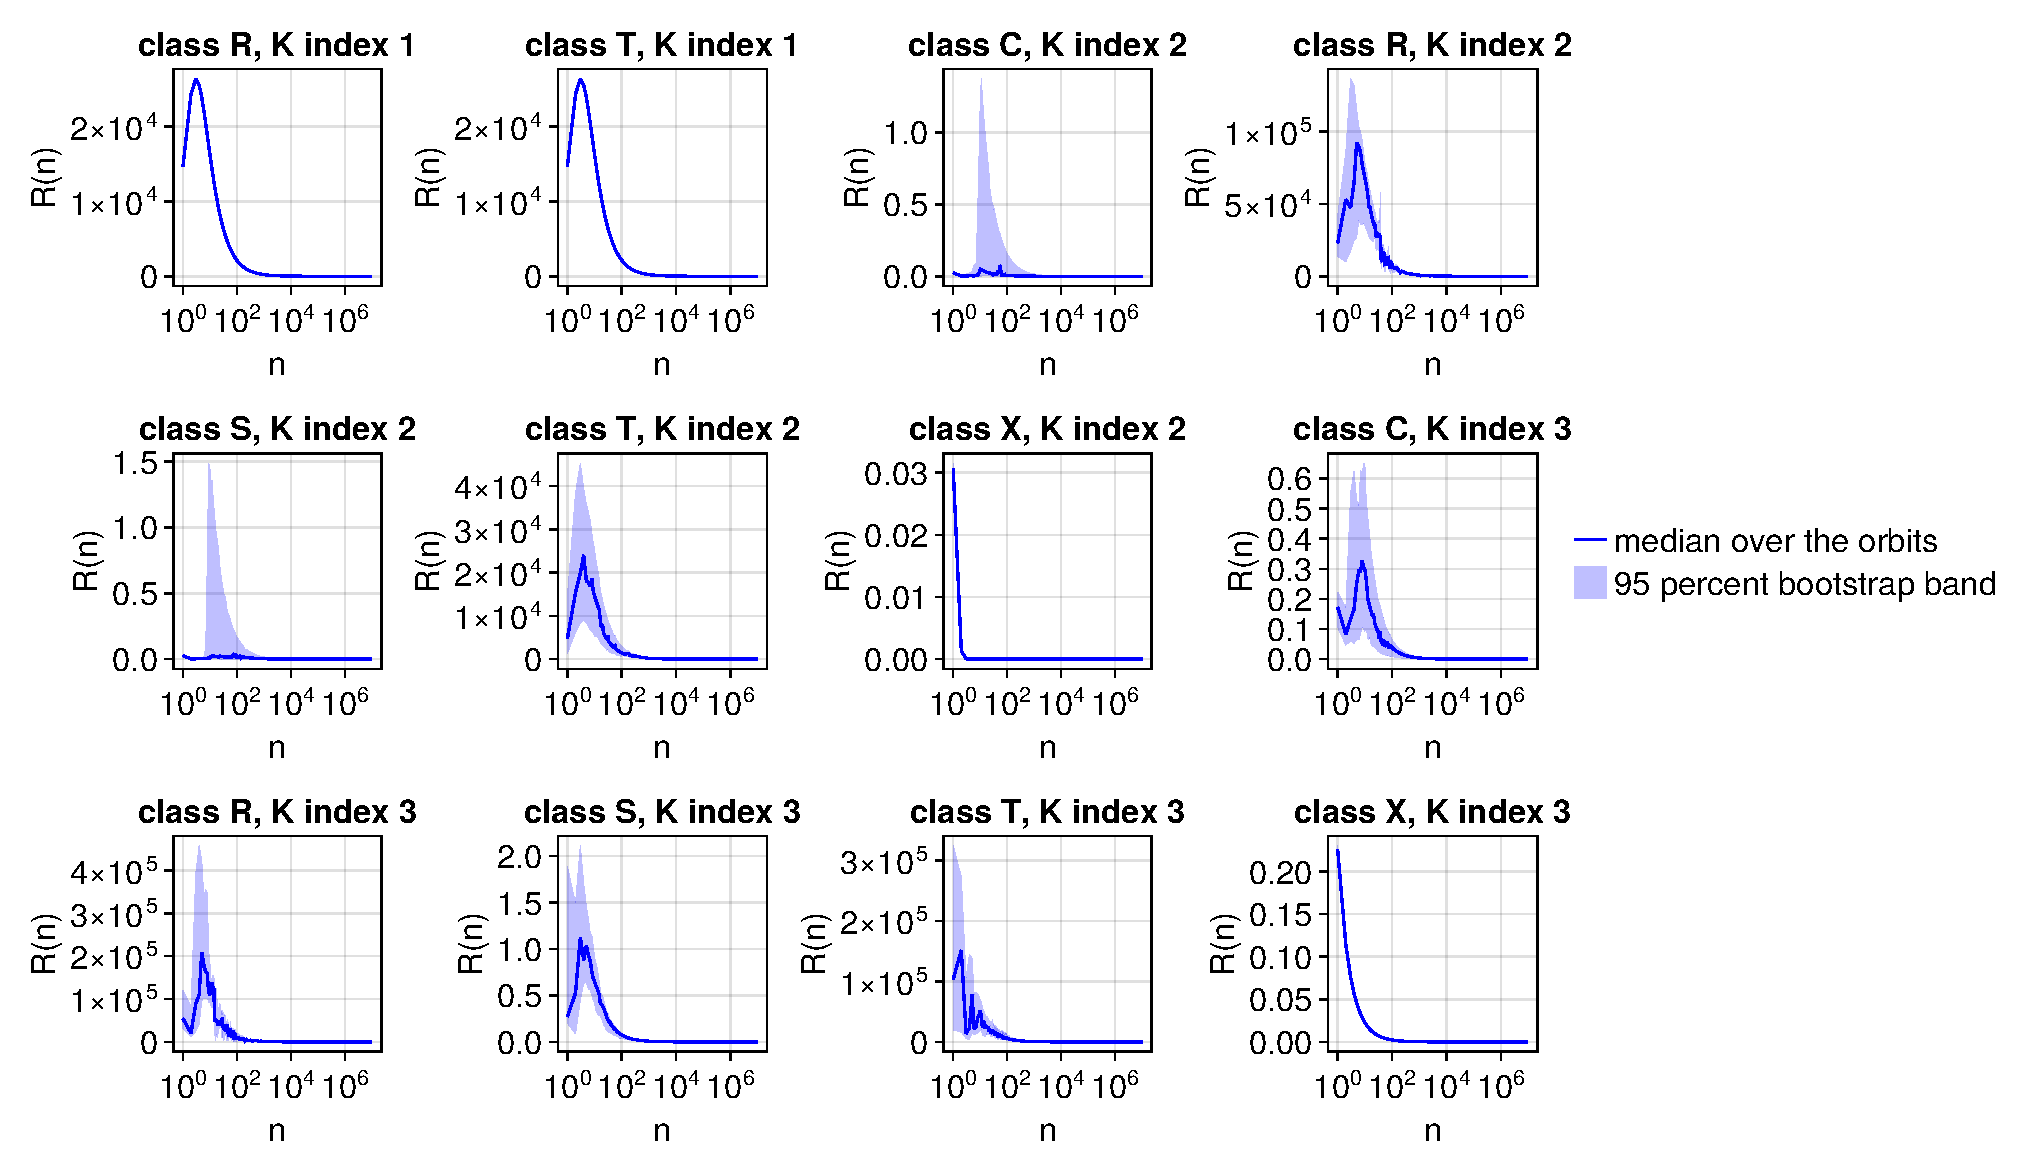
\includegraphics[width=\textwidth]{../figures/p1-le-benchmark-fig-F2a.pdf}
\caption{Median of $R(n)$ over the orbits of each cell and over the pooled set $W$, with the 95 percent bootstrap band, $K$ index 1 to 3.}
\label{fig:F2}
\end{figure*}

\begin{figure*}
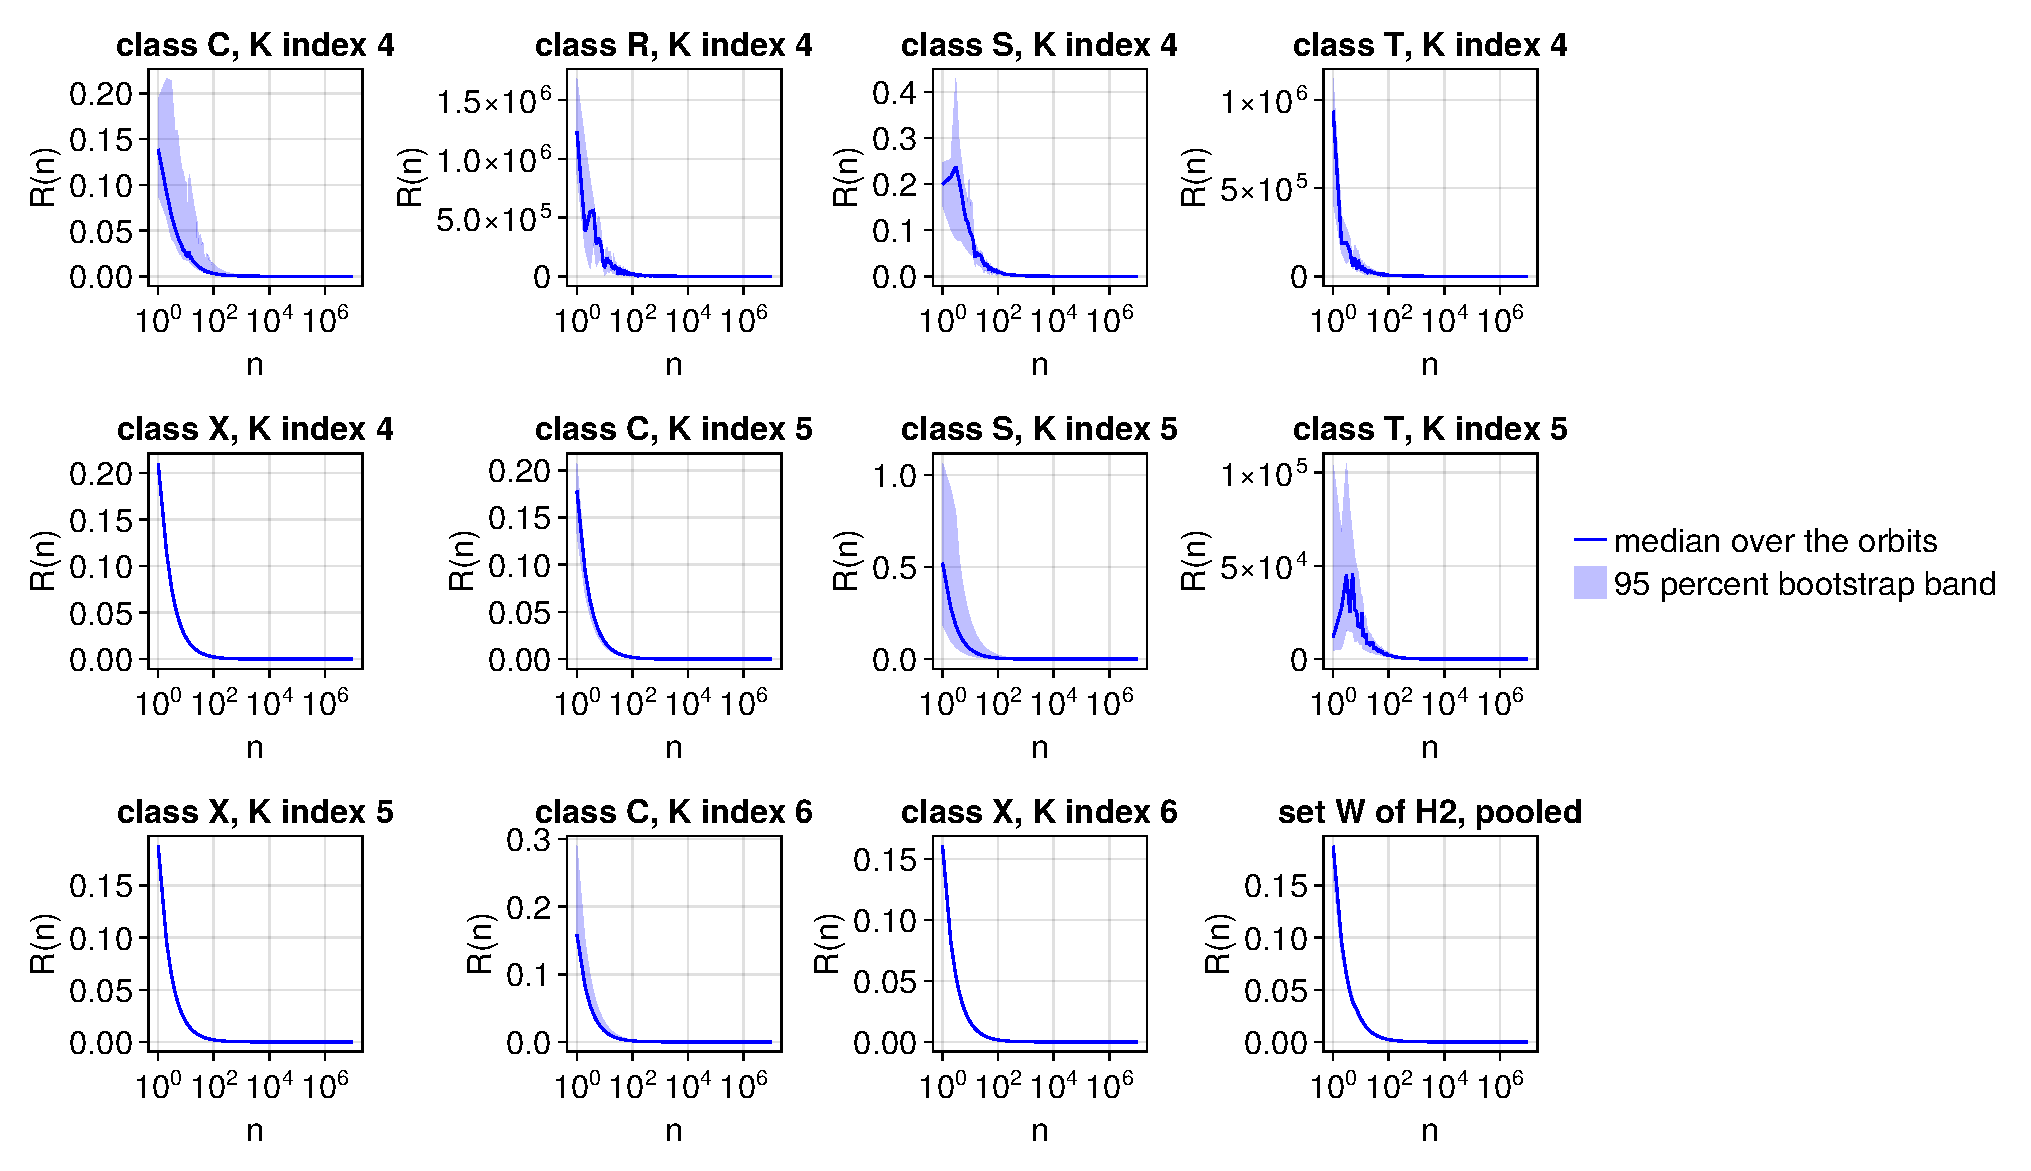
\includegraphics[width=\textwidth]{../figures/p1-le-benchmark-fig-F2b.pdf}
\caption{As Fig.~\ref{fig:F2}, for $K$ index 4 to 6 and the pooled set $W$.}
\label{fig:F2b}
\end{figure*}

\section{Results for H3 (claim C2): SUPPORTED}
\label{sec:h3}

\subsection{Preregistered rule}
\label{sub:h3rule}

\nconv\ is the smallest $n$ after which every method stays within a 0.05 relative band of $\lref$ up to $N$.
Per orbit it is the maximum over the methods of $V$:
\begin{align}
\nconv &= \max_{m\in V}\nconv^{(m)},\\
\nconv^{(m)} &= \min\bigl\{n:\ |\lambda_m(n')-\lref|\le 0.05\,|\lref|\nonumber\\
&\qquad\text{for all recorded } n'\in[n,N]\bigr\}.
\end{align}
H3 is SUPPORTED if the ratio of the median \nconv\ over $W$ to the median \nconv\ over the strong-chaos set $S$ is at least 10, and the lower end of the 95 percent bootstrap interval of the ratio is above 3.
Here $W$ is the set of \Sec{sub:notation} and $S$ is the class C orbits at $K=2\pi$ and $K=10$.
Orbits whose \nconv\ is undefined are given $\nconv=N$, and their share is reported.

\subsection{Measured}

Table~\ref{tab:h3} gives the H3 measured values.

\begin{table*}
\caption{H3 measured values.}
\label{tab:h3}
\begin{ruledtabular}
\begin{tabular}{lcc}
Quantity & Value & Threshold \\
\hline
Orbits in $W$ & 355 & \\
Orbits in $S$ & 80 & \\
Median \nconv\ over $W$ & \sci{2.511886}{6} & \\
Median \nconv\ over $S$ & 224.0 & \\
Ratio & 11213.7767857 & at least 10 \\
95 percent bootstrap interval of the ratio & [7924.465, 14117.3125] & lower end above 3 \\
Share of undefined \nconv & 0.0229885057471 & \\
$S$ orbits without positive growth & 0 & \\
\end{tabular}
\end{ruledtabular}
\end{table*}

H3 is supported.
The analysis code reports the verdict supported.
Both conditions pass.
The ratio is at least 10 and the lower end is above 3.
The strong-chaos set $S$ of H3 is the class C orbits at $K=2\pi$ and $K=10$.
It is not the panel class S.
The orbits with undefined \nconv\ enter the medians at the value $N$.
Table~\ref{tab:h3cell} gives \nconv\ by cell.
The rows of class C at $K$ index 5 and 6 are the orbits of $S$.
The other rows match the cells of Table~\ref{tab:h2cell} in class, $K$ index and orbit count.
The cell-level medians are descriptive.
The class S cell at $K$ index 5 has 1 orbit and is not decidable, as in H2.

\begin{table*}
\caption{H3: \nconv\ by cell (descriptive).}
\label{tab:h3cell}
\begin{ruledtabular}
\begin{tabular}{llccccl}
Class & $K$ index & Orbits & Median & Lo & Hi & Note \\
\hline
C & 2 & 36 & \sci{7.079458}{6} & \sci{6.309573}{6} & \sci{7.943282}{6} & \\
S & 2 & 21 & \sci{7.079458}{6} & \sci{5.0}{6} & \sci{7.079458}{6} & \\
X & 2 & 36 & \sci{7.079458}{6} & \sci{5.623413}{6} & \sci{7.079458}{6} & \\
C & 3 & 34 & \sci{4.223954}{6} & \sci{3.03001}{6} & \sci{6.309573}{6} & \\
S & 3 & 37 & \sci{5.623413}{6} & \sci{3.548134}{6} & \sci{7.943282}{6} & \\
X & 3 & 36 & \sci{5.623413}{6} & \sci{3.981072}{6} & \sci{6.6945155}{6} & \\
S & 4 & 37 & 794328.0 & 707946.0 & \sci{1.0}{6} & \\
X & 4 & 37 & 63096.0 & 44668.0 & 89125.0 & \\
C & 5 & 40 & 266.5 & 200.0 & 335.5 & \\
S & 5 & 1 & 501187.0 & 501187.0 & 501187.0 & not decidable \\
X & 5 & 40 & 251.0 & 168.0 & 447.0 & \\
C & 6 & 40 & 212.0 & 178.0 & 251.0 & \\
X & 6 & 40 & 158.0 & 133.5 & 224.0 & \\
\end{tabular}
\end{ruledtabular}
\end{table*}

Figure~\ref{fig:F3} shows the \nconv\ distributions.

\begin{figure}
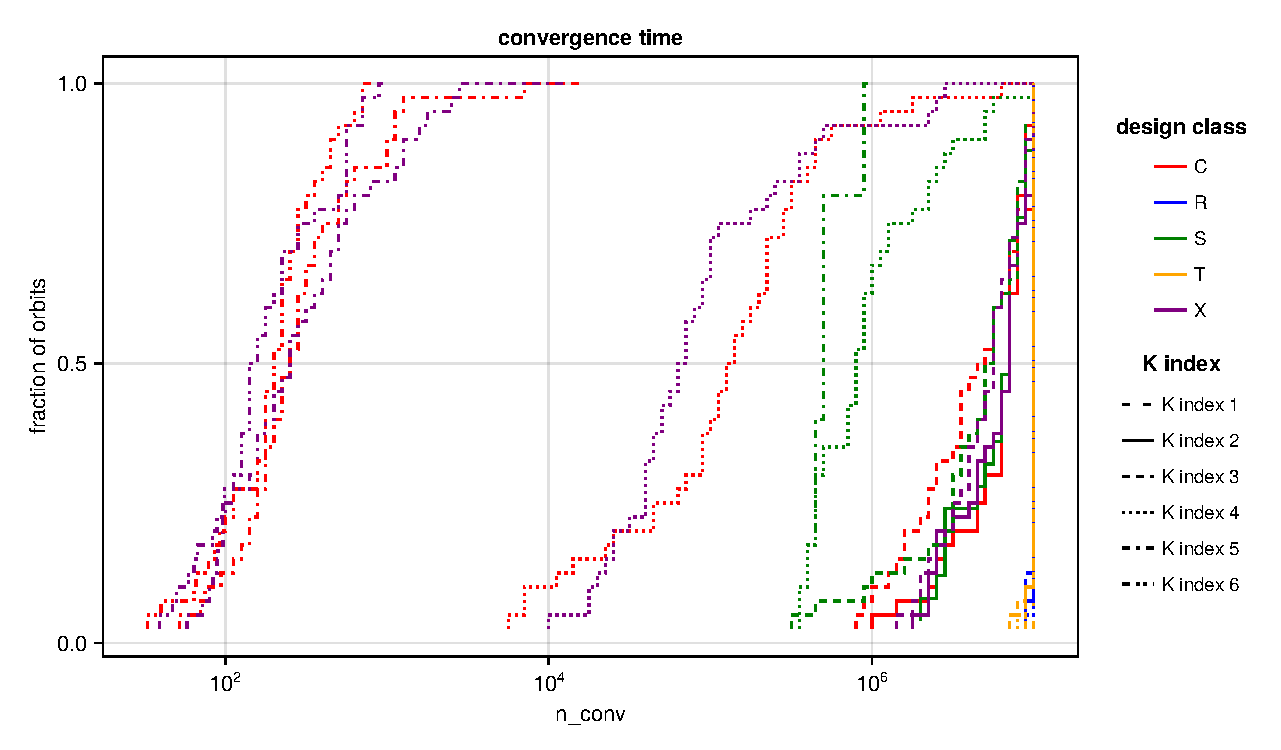
\includegraphics[width=\columnwidth]{../figures/p1-le-benchmark-fig-F3.pdf}
\caption{Empirical distribution functions of \nconv\ per cell; colour by design class, line style by $K$ index.}
\label{fig:F3}
\end{figure}

\section{Results for H4 (REPRODUCES, Sala and Artuso \cite{SalaArtuso2015}): DID NOT REPRODUCE}
\label{sec:h4}

\subsection{Preregistered rule}

The start is $x_0=$\tenp{-3} and $p_0=-$\tenp{-3}, with $T=$\tenp{9} iterations.
At $K=\pi/2$ (reference 0.298) both L1 and L5 (Float64, $\tau=1$) must be within 0.01.
At $K=2\pi$ (reference 1.172) both must be within 0.02.
The reference values are those of Sala and Artuso \cite{SalaArtuso2015}.
H4 is SUPPORTED if both $K$ pass.
A failure is reported as ``did not reproduce'' with the numbers.

\subsection{Measured}

The analysis code reports the verdict did not reproduce.
Table~\ref{tab:h4} gives the verdict table.

\begin{table*}
\caption{H4 verdict table.}
\label{tab:h4}
\begin{ruledtabular}
\begin{tabular}{lccccc}
Start & L1 & L5 & Reference & Tolerance & Pass \\
\hline
$K=\pi/2$ & 0.256066843848 & 0.256066843848 & 0.298 & 0.01 & false \\
$K=2\pi$ & 1.17018723872 & 1.17018723872 & 1.172 & 0.02 & true \\
\end{tabular}
\end{ruledtabular}
\end{table*}

H4 did not reproduce.
At $K=\pi/2$ both L1 and L5 gave 0.256066843848 against the reference 0.298.
The value lies below the reference and outside the tolerance of 0.01.
The $K=\pi/2$ start did not reproduce the published value \cite{SalaArtuso2015}.
At $K=2\pi$ the value 1.17018723872 against 1.172 is within the tolerance of 0.02.
The reproduction as a whole fails.
The possibility that the orbit of the published paper sits in a different component remains open.
The analysis does not decide it.
Each $K$ rests on one start, with no error bar.

\subsection{Comparators (no verdict)}
\label{sub:comp}

Table~\ref{tab:comp} gives three comparators at the five $K$ values: the ensemble mean of $\lam{L5}(N_1)$ over the kept chaotic-sea orbits, the fit of Shevchenko \cite{Shevchenko2014}, and the line $\ln(K/2)$ \cite{Chirikov1979}.
They never pass or fail.
The frozen text designates the line for $K=\pi/2$, $2\pi$ and 10.
The analysis code reports it at all five $K$.
The rows at $K=0.5$ and $K=\Kc$ lie outside the designated $K$ and are shown as reported; the line takes negative values there ($-1.38629436112$ and $-0.721921822156$).
The range of applicability of the fit and of the line is not checked in this paper.
No verdict is attached to any comparator row.

\begin{table*}
\caption{Comparators.}
\label{tab:comp}
\begin{ruledtabular}
\begin{tabular}{llcccc}
$K$ index & $K$ & Orbits & Mean & Shevchenko fit & $\ln(K/2)$ \\
\hline
2 & 0.5 & 40 & 0.0575923614667 & 0.06665 & $-1.38629436112$ \\
3 & 0.971635406 & 40 & 0.091095497804 & 0.12951899962 & $-0.721921822156$ \\
4 & 1.57079632679 & 40 & 0.298004458001 & 0.342657808664 & $-0.24156447527$ \\
5 & 6.28318530718 & 40 & 1.17214446011 & 1.17006018176 & 1.14472988585 \\
6 & 10 & 40 & 1.62000488786 & 1.61943791243 & 1.60943791243 \\
\end{tabular}
\end{ruledtabular}
\end{table*}

\subsection{Exploratory item E4 (EXPLORATORY)}
\label{sub:h4exp}

E4 (EXPLORATORY): H4 at the shorter horizon.
The cross-check uses $T=$\tenp{8}.
It has no verdict under the frozen rule.
E4 does not change the H4 verdict, which stands under the frozen rule: H4 did not reproduce.
At $K=\pi/2$ it gives 0.299256534631 (Float64) and 0.299012763029 (Double64).
At $K=2\pi$ it gives 1.17243899416 and 1.17179404609.
The Float64 value at $K=\pi/2$ at $T=$\tenp{9} in the verdict table is 0.256066843848.
The ensemble mean of $\lam{L5}(N_1)$ over the 40 kept chaotic-sea orbits at $K=\pi/2$ is 0.298004458001.
The analysis does not show why the single start at $K=\pi/2$ gives a different value at $T=$\tenp{9} than at $T=$\tenp{8}.
No cause is claimed.

\section{Results for H5: SUPPORTED}
\label{sec:h5}

\subsection{Preregistered rule}

On the ladder subset $S_L$, H5a is the fraction of $S_L$ orbits whose two labels are identical at Float64, Double64 and BigFloat.
It must be at least 0.90.
H5b is the fraction of all panel orbits with either axis ``unresolved''.
It must be at most 0.30.
H5c is the fraction with structure ``unresolved'' among orbits with instability ``none detected on the tested horizon''.
It must be at most 0.30.
H5 is supported only if all three sub-rules pass.
H5a is read from the per-precision labels before the ladder test acts.

\subsection{Measured}

The analysis code reports the verdict supported.
Table~\ref{tab:h5} gives the three sub-rules.

\begin{table}
\caption{H5 sub-rules.}
\label{tab:h5}
\begin{ruledtabular}
\begin{tabular}{lcccc}
Sub-rule & Orbits & Fraction & Limit & Result \\
\hline
H5a & 92 & 1.0 & at least 0.90 & pass \\
H5b & 883 & 0.0951302378256 & at most 0.30 & pass \\
H5c & 334 & 0.0568862275449 & at most 0.30 & pass \\
\end{tabular}
\end{ruledtabular}
\end{table}

All three label conditions are met.
H5 is supported under its three sub-rules.

\subsection{Exploratory items E3 and E5 (EXPLORATORY)}
\label{sub:h5exp}

E3 (EXPLORATORY): H5a is 1.0 while many ladder labels are forced.
H5a is 1.0 on 92 $S_L$ orbits, read before the ladder test acts.
The ladder test then forced the labels of 35 of those 92 orbits to unresolved, a share of 0.380434782609.
Both hold at once: the per-label agreement across precisions, and the override of 35 labels by the ladder test.
The analysis code reports the unresolved share before the tests as 46 of 883 (0.0520951302378) and after as 84 of 883 (0.0951302378256).
The second value is the H5b fraction.
Other forced tests: direction 7 of 172 (0.0406976744186).
Estimator, diagnostics and excluded show 0 of 883 each.
The analysis does not show how the forced counts (35 and 7) relate to the rise from 46 to 84.
No cause is claimed.
Figure~\ref{fig:F4} shows the share of orbits forced by each label test.

\begin{figure}
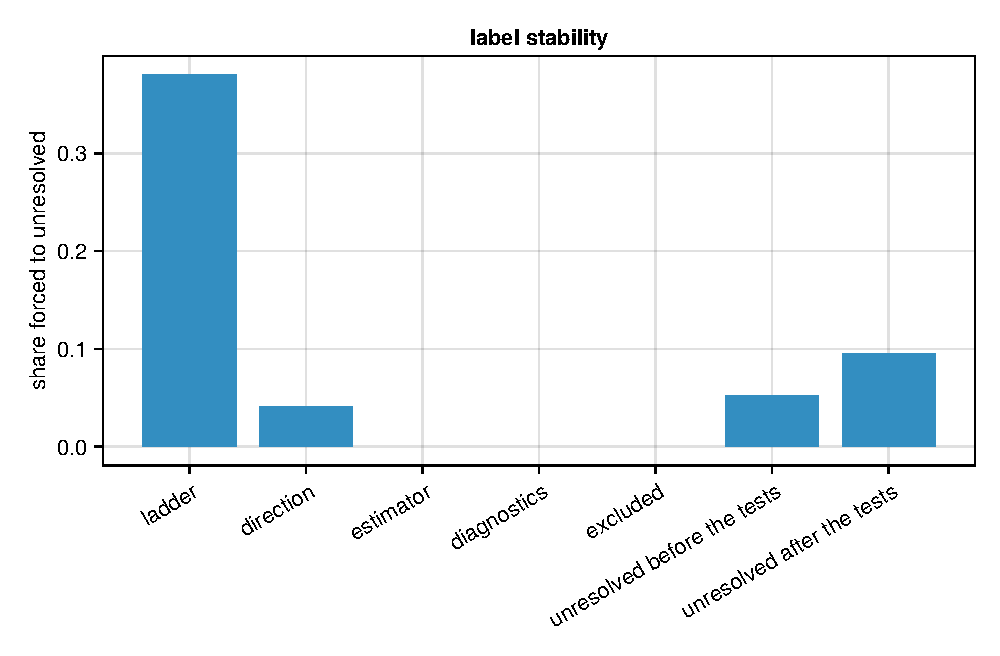
\includegraphics[width=\columnwidth]{../figures/p1-le-benchmark-fig-F4.pdf}
\caption{Share of orbits forced to unresolved by each label test, among the orbits the test applies to, and the share of all orbits unresolved before and after the tests.}
\label{fig:F4}
\end{figure}

E5 (EXPLORATORY): unresolved labels by cell.
``Both'' counts orbits with both axes unresolved (65 in all).
``Structure only'' counts orbits with instability ``none detected on the tested horizon'' and structure unresolved (19 in all).
The two add to the 84 of H5b.
Cells not listed in Table~\ref{tab:unres} have none.

\begin{table}
\caption{Unresolved labels by cell (EXPLORATORY).}
\label{tab:unres}
\begin{ruledtabular}
\begin{tabular}{llccc}
$K$ index & Class & Cell orbits & Both & Structure only \\
\hline
0 & controls & 13 & 3 & 0 \\
2 & C & 40 & 4 & 0 \\
2 & R & 40 & 5 & 0 \\
2 & S & 25 & 4 & 0 \\
2 & T & 40 & 0 & 11 \\
2 & X & 40 & 4 & 0 \\
3 & C & 40 & 6 & 0 \\
3 & R & 40 & 6 & 0 \\
3 & S & 40 & 3 & 0 \\
3 & T & 40 & 2 & 5 \\
3 & X & 40 & 4 & 0 \\
4 & C & 40 & 2 & 0 \\
4 & R & 40 & 6 & 1 \\
4 & S & 40 & 3 & 0 \\
4 & T & 40 & 2 & 2 \\
4 & X & 40 & 3 & 0 \\
5 & S & 5 & 4 & 0 \\
5 & T & 40 & 4 & 0 \\
\end{tabular}
\end{ruledtabular}
\end{table}

$K$ index 1, $K$ index 6 and $K$ index 5 classes C and X have no unresolved orbit.

\section{Cost and sensitivity (reported without a decision rule)}
\label{sec:cost}

Symplectic residuals $\epsilon_{\mathrm{pair}}(n)$ and $\epsilon_{\mathrm{det}}(n)$ are shown in Fig.~\ref{fig:F5} only.
No numbers for them are quoted.

\begin{figure*}
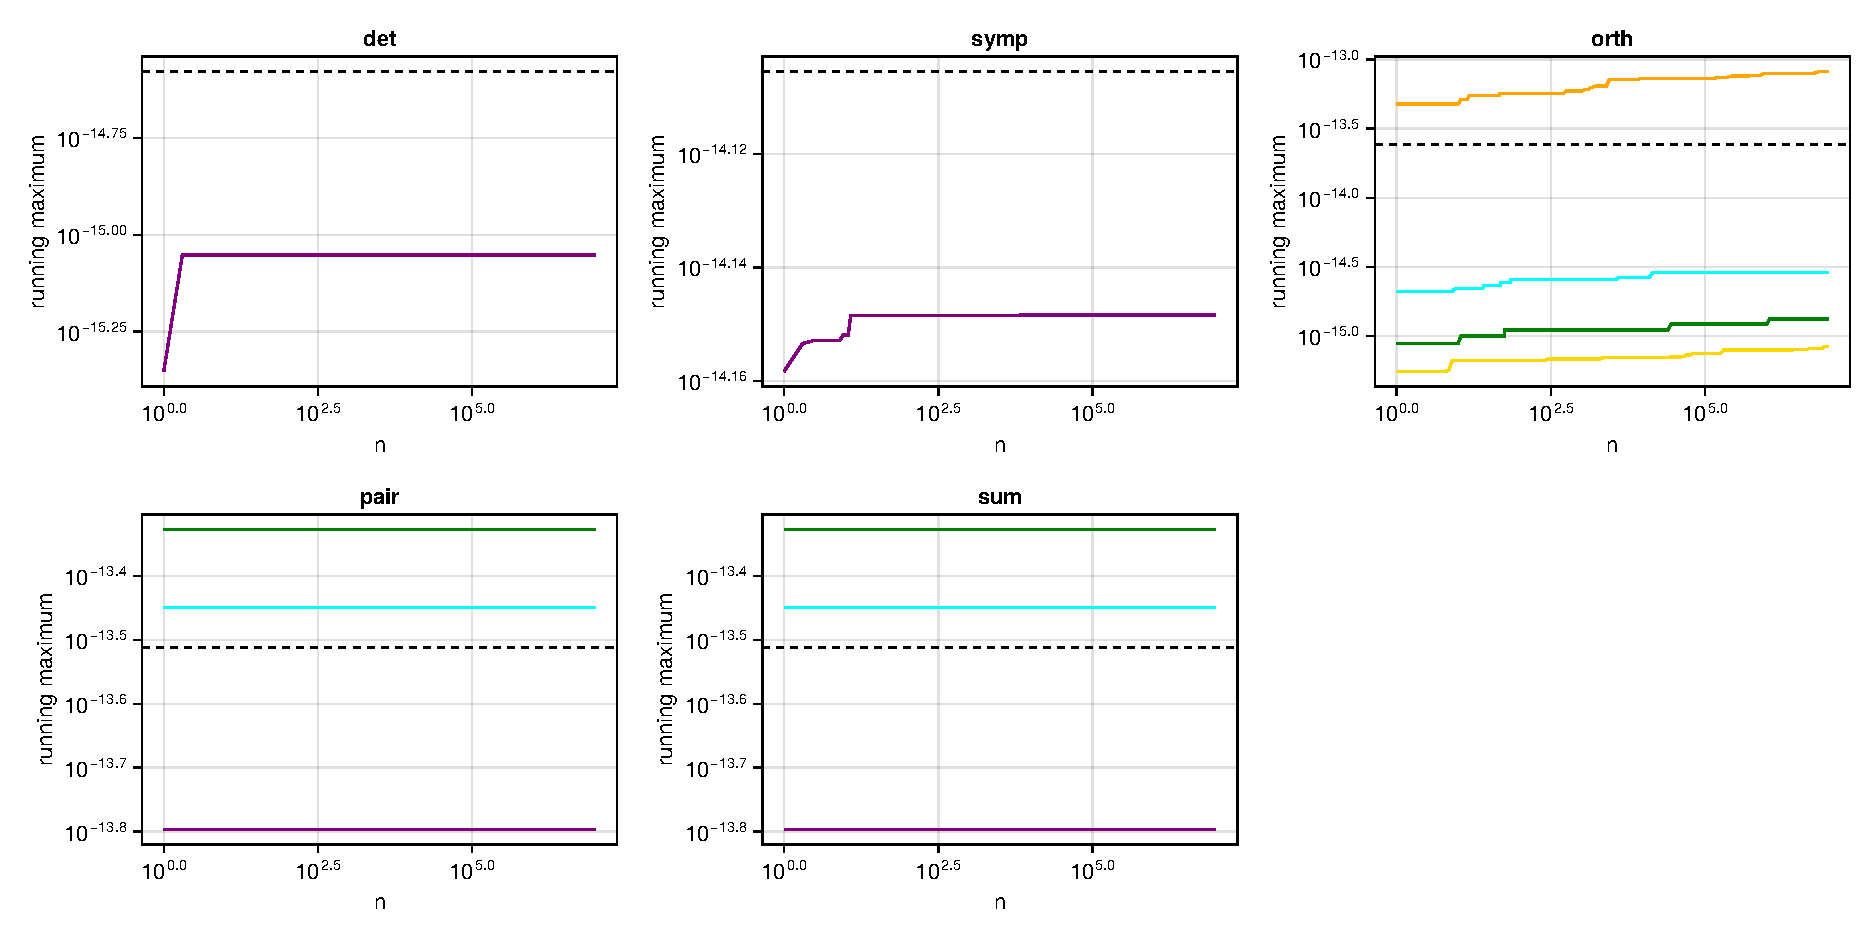
\includegraphics[width=\textwidth]{../figures/p1-le-benchmark-fig-F5.pdf}
\caption{Largest running maximum over the orbits of each stored diagnostic (det, symp, orth, pair, sum) per method, with the median threshold over the orbits; each orbit is tested against its own threshold.}
\label{fig:F5}
\end{figure*}

\subsection{Cost}

Table~\ref{tab:cost} gives ns per orbit-step by method and precision, and relative to L5 in the same precision.
Each row is an unweighted mean over all items of that method and precision, so the item sets differ between rows.
Relative to L5 in Float64 (168.60570837 ns per orbit-step), L1 costs 0.701549448499, L2 0.503966109187, L4 0.982175001597, L9 1.23876330018 and L6 2.10273197634.
These ratios compare rows with different item sets (1917, 1571, 1915, 1915 and 1227 items against 2605 for L5), and they come from a single run that used 23 of 23 available threads, with no repeated timing reported.
L5 costs 4882.6924383 ns in Double64 and 377399.856865 ns in BigFloat(256).
The Double64 and BigFloat rows have 186 and 92 items against 2605 for L5 in Float64, so they are also not like-for-like with the Float64 rows.
Figure~\ref{fig:F6} shows the thread nanoseconds per orbit-step.

\begin{table*}
\caption{Cost per orbit-step.}
\label{tab:cost}
\begin{ruledtabular}
\begin{tabular}{llccc}
Method & Precision & Items & ns per orbit-step & Relative to L5 \\
\hline
L5 & Float64 & 2605 & 168.60570837 & 1.0 \\
L1 & Float64 & 1917 & 118.285241721 & 0.701549448499 \\
L2 & Float64 & 1571 & 84.9715628342 & 0.503966109187 \\
L4 & Float64 & 1915 & 165.600311888 & 0.982175001597 \\
L9 & Float64 & 1915 & 208.86256373 & 1.23876330018 \\
L6 & Float64 & 1227 & 354.532614384 & 2.10273197634 \\
L5 & Double64 & 186 & 4882.6924383 & 1.0 \\
L5 & BigFloat(256) & 92 & 377399.856865 & 1.0 \\
\end{tabular}
\end{ruledtabular}
\end{table*}

\begin{figure}
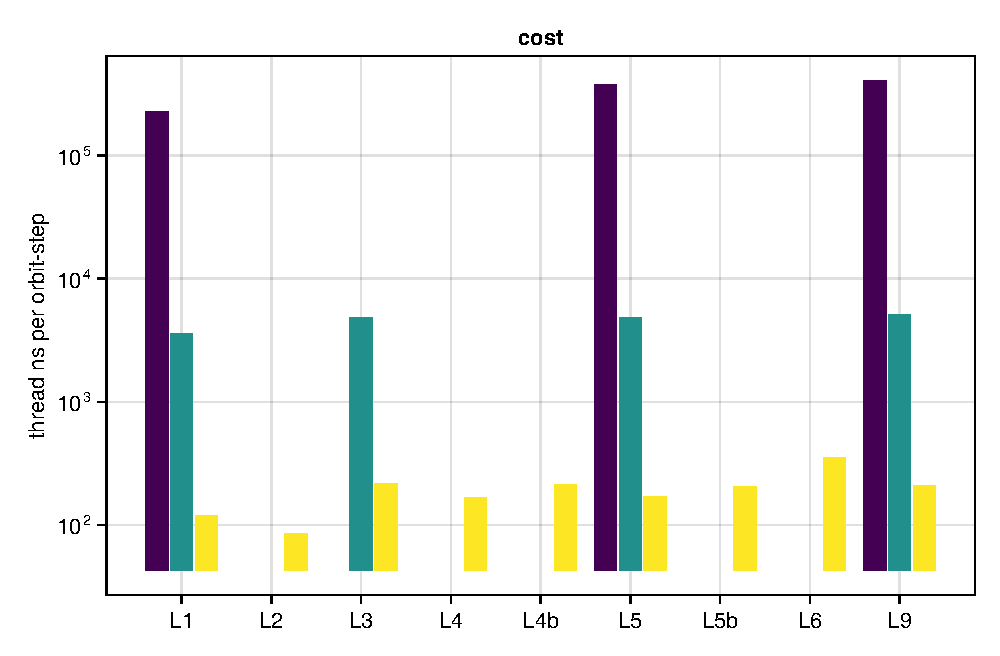
\includegraphics[width=\columnwidth]{../figures/p1-le-benchmark-fig-F6.pdf}
\caption{Thread nanoseconds per orbit-step by method and precision.}
\label{fig:F6}
\end{figure}

Run totals: the total wall time was 11957.993616580963 seconds against a cap of 12.0 hours.
The plan had 1363 chunks and 15569 items.
The run used 23 threads of 23 available.
All 13 arms are complete.

\subsection{Sensitivity}

The sensitivity analysis has 31 rows.
The column is the median paired difference of $\lambda$ at \nH\ against the primary item, with 171 orbits per row except the $\tau$ rows.
These rows are evaluated at $\nH=$\tenp{4}.
H1c is evaluated at $N_1=$\tenp{7}.
The rows below are therefore not an evaluation of the H1c result.
Figure~\ref{fig:F7} shows the rows.

\begin{figure*}
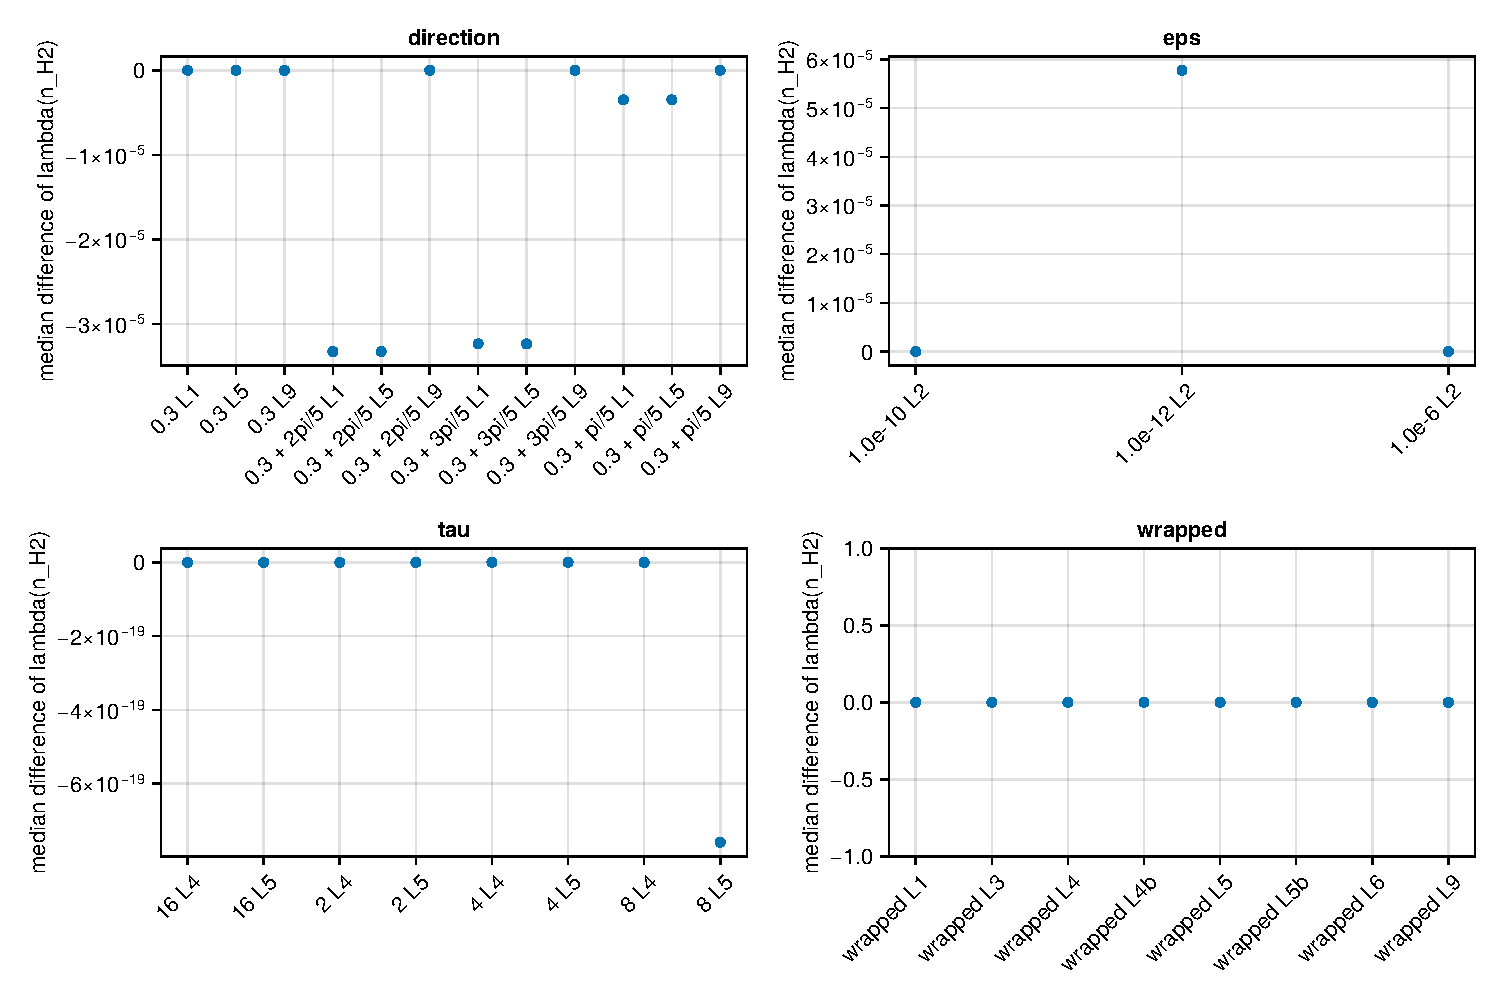
\includegraphics[width=\textwidth]{../figures/p1-le-benchmark-fig-F7.pdf}
\caption{Median paired difference of $\lambda(\nH)$ from the primary item for the levels of $\tau$, $\epsilon$, initial direction and coordinate mode, over the kept $S_D$ orbits.}
\label{fig:F7}
\end{figure*}

Direction.
L1 and L5 values are of order \tenp{-9} at offset 0.3 ($\lam{L5}=$\sci{1.73141166638}{-9}).
They are of order \tenp{-5} or \tenp{-6} at the other offsets: $\lam{L5}$ is $-$\sci{3.32612943661}{-5} at $0.3+2\pi/5$, $-$\sci{3.23438506002}{-5} at $0.3+3\pi/5$ and $-$\sci{3.48457834277}{-6} at $0.3+\pi/5$.
L9 is 0.0 in every direction row.

The $\epsilon$ rows for L2.
With $\epsilon=$\tenp{-10} the value is \sci{2.26005874629}{-9}.
With $\epsilon=$\tenp{-12} it is \sci{5.77729472453}{-5}.
With $\epsilon=$\tenp{-6} it is \sci{4.04116577712}{-10}.

Wrapped versus lifted is 0.0 for all eight methods of $V$.
The column \texttt{median\_log10\_nconv\_ratio} is 0.0 in all 31 rows.
This is reported as printed.
It has not been checked whether a constant column is an artefact.

Tau sweep.
$\tau=2$ and 4 show no breakdown, with 171 orbits for L4 and L5.
$\tau=8$ has 154 orbits for L4 and L5, with breakdown count 17.
$\tau=16$ has 132 orbits for L4 with breakdown count 39 and 134 orbits for L5 with breakdown count 37.
At $\tau=16$ the breakdown steps are 16 or 32 for L4 and 16 to 288 for L5.

\section{Exploratory results}
\label{sec:expl}

All items in this section are EXPLORATORY.
They are not confirmatory, have no frozen rule and carry no claimed cause.
Items E1 to E5 appear in \Sec{sec:h1}, \Sec{sec:h4} and \Sec{sec:h5}, where they bear on a hypothesis.
E6 and E7 are reported here.

E6 (EXPLORATORY): short, empty and not decidable cells.
The panel record marks two cells as short (``fewer qualifying grid cells than $n_c$''): $K$ index 2 class S (25 drawn, 25 qualifying) and $K$ index 5 class S (5 drawn, 5 qualifying).
It marks as empty $K$ index 5 class R (no elliptic periodic point) and $K$ index 6 classes R (no elliptic periodic point), T and S (no qualifying grid cell).
It marks $K$ index 1 classes C, S and X as undefined (class undefined at $K=0$).
Class X shows 0 qualifying grid cells at every $K$ index from 2 to 6.
The preregistered selection rule does not draw class X from the screening and places the starts near the hyperbolic fixed point.
In the H2 and H3 tables only class S at $K$ index 5 is not decidable, with 1 orbit.

E7 (EXPLORATORY): cell patterns.
The largest cell median of $R(\nH)$ is 0.000775501992792 (class S, $K$ index 3).
The smallest is \sci{5.82402750446}{-12} (class X, $K$ index 2).
Both are in Table~\ref{tab:h2cell}.
The cell medians of \nconv\ are between \sci{4.223954}{6} and \sci{7.079458}{6} at $K$ index 2 and 3.
The horizon there is $N_1=$\tenp{7}.
These values are in Table~\ref{tab:h3cell}.
At $K$ index 4 they are 794328.0 (class S) and 63096.0 (class X).
At $K$ index 5 and 6 they lie between 158.0 and 266.5, excluding class S at $K$ index 5.
Several cells share the same median (for example \sci{7.079458}{6} in three cells of Table~\ref{tab:h3cell}), which is consistent with \nconv\ taking recorded values of $n$ (\Sec{sub:notation}).
The effect of this resolution on the bootstrap intervals is not examined.
The analysis does not show why.

\section{Limitations}
\label{sec:lim}

\begin{enumerate}
\item The study rests on one draw of the panel (a single seed) with 883 orbits.
The bootstrap intervals resample orbits within that draw, treat the orbits as independent resampling units, and do not reflect a second draw.
The cell tables of H2 and H3 are descriptive.
The composition of the 883 orbits is given in \Sec{sub:panel}.
\item The panel is run in Float64 only.
Precision comparisons come from the ladder subset $S_L$ of 92 orbits, and H5a rests on that subset.
\item A set or cell with fewer than 20 orbits is not decidable and is neither pass nor fail.
In the H2 and H3 tables only class S at $K$ index 5 (5 drawn, 1 in $W$) is below that minimum.
Class S at $K$ index 2 has 25 drawn and 21 in $W$, which is above the minimum.
Cell-level medians and intervals are descriptive, and the decisions use the pooled sets.
H4 rests on one start per $K$, as the frozen text specifies, with no error bar.
\item L2 runs in wrapped coordinates.
This affects the H1c metric, the sub-rule that failed.
The analysis does not show whether this accounts for any part of the H1c result.
\item The numbers were checked against the output of the analysis run.
The analysis code was verified against an independent recomputation.
The numbers were not recomputed from the stored series for this paper.
Figures~\ref{fig:F1} to~\ref{fig:F7} were redrawn and viewed; they plot the figure data of the analysis output, unchanged.
\item $W$ is defined here by the preregistration.
The analysis code still reports a shorter phrase for $W$ in its list of readings (class C at $0<K\le\Kc$), which does not describe the cells of Tables~\ref{tab:h2cell} and~\ref{tab:h3cell}; the membership of $W$ (355 orbits) does not depend on that phrase.
\item The list of controls with positive analytic exponent has 10 of the 13 controls; the other 3 are the elliptic controls with exponent 0, which no decision rule of H1 uses (\Sec{sub:ctrl}).
Orbit 881 is an info control and the orbit dropped as drift.
\item Table~\ref{tab:run} gives two git commits, one for the run and one for the analysis.
They are related through the repository history only; the study manifests record each commit separately and no single run record names both.
\item The run outputs are excluded from version control, so they are not part of the repository (see Data availability).
The stored series are packed for deposit as a dataset on Zenodo (1363 chunk files with the manifest, the panel, the preregistration, the parameter file, the file-format description and a SHA-256 list); the dataset DOI is given in the Data availability section once it is issued.
\item The frozen preregistration is in the repository (see Data availability).
No external time-stamped deposit of it is recorded.
\item Cost values come from a single run in which 23 of 23 available threads were used, with no repeated timing reported.
The item sets differ between rows, and the Double64 and BigFloat rows have 186 and 92 items.
The cost ratios are therefore not controlled comparisons.
\item \nconv\ takes recorded values of $n$, because the series are stored at 20 points per decade, log-spaced, plus the first 100 steps.
Its resolution and its effect on the bootstrap intervals are not examined.
\item The column \texttt{median\_log10\_nconv\_ratio} is 0.0 in all 31 sensitivity rows.
It has not been checked whether this is an artefact.
\item Open items: the analysis code keeps a constant named STRONG\_K, and its role is not described in this paper.
The package requires Julia 1.11 or later, so no dependency manifest for Julia 1.10 is kept.
\end{enumerate}

\section{Conclusion}
\label{sec:concl}

Scope: one panel from a single draw (a single seed), run in Float64, with five nonzero kick values and one start per kick value in H4 (\Sec{sec:lim}).

Under the preregistered rules, H1 (claim C1) is falsified, on sub-rule H1c alone, with H1a and H1b met in full.
It was evaluated in Float64 at $N_1=$\tenp{7}, with L2 in wrapped coordinates (limitation~4).

Claim C2 has two preregistered tests with different verdicts.
H2 (claim C2) is not supported (NEGATIVE).
It measures $R(\nH)=\Delta_V(\nH)/\lref$ over the set $W$ at $\nH=$\tenp{4} steps.
H3 (claim C2) is supported.
It compares the median \nconv\ over $W$ with the median \nconv\ over the strong-chaos set $S$, where \nconv\ is the maximum over $V$ of the smallest $n$ after which a method stays within a 0.05 relative band of $\lref$.
This paper does not combine the two verdicts into one verdict on C2.

H4 did not reproduce the published value at $K=\pi/2$ and passed at $K=2\pi$.
H5 is supported under its three sub-rules (H5a, H5b, H5c).
The ladder test forced 35 of the 92 ladder-subset labels to unresolved (exploratory item E3).
H4 and H5 are not tied to C1 or C2.

TOOL: Chaoslab v0.1.1 is a tagged and documented release of the code the run used; every method of the run is \texttt{verified} (\Sec{sub:prereg} and the Data availability section).

\begin{acknowledgments}
Drafting, adversarial review and revision of this manuscript, and the analysis code, were done with Claude models (Anthropic, Claude Sonnet 5.5) operated through Claude Code under the direction of the author.
The author decided the scope, the framing and the preregistered rules, and accepted or redirected the output at each stage checkpoint.
Numbers in the text were copied from an analysis output produced by the analysis code, which was checked against an independent recomputation.
Citations are limited to entries verified in the project bibliography.
The author is responsible for the content.
\end{acknowledgments}

\section*{Author declarations}

\subsection*{Conflict of interest}

The author has no conflicts to disclose.

\subsection*{Author contributions}

georgehadji: Conceptualization; Methodology; Software; Validation; Formal analysis; Investigation; Data curation; Writing - original draft; Writing - review and editing; Visualization.

\section*{Data availability}

The repository is \url{https://github.com/georgehadji/Chaos} (GPL-3.0-or-later).
The frozen preregistration is in the repository.
Its header SHA-256 is \hash{62011ba5af514da4f1238aef9ae6cb35ca21093c4343b71dd696df360b9994bf} (Table~\ref{tab:run}).
The git SHA at freeze recorded in its header is \hash{1e760e229eabf9d8323ad4d8097cc1dbd017f845}, the parent commit of the freeze commit.
Amendments A1 to A6 are in the same file and in its amendment log.

The numbers in this paper come from one analysis run at commit \hash{d31b655d0c33e2f2f1a67bbbdeba9c8c8a3fd036}.
The stored series come from the run at commit \hash{3e405f3324f8d25162580d3380db26c877d7ca63}, an ancestor of the analysis commit with the same series code (\Sec{sub:run}).
The figures were drawn from the figure data of the analysis output by the figure extension of the repository at commit caaf95a; the figure data are those of the study output, unchanged.
The study manifest has SHA-256 \hash{ae6ec80eb08fbd6e98aeef1fbf840a567a03102ab943f2ae0aaf2b3e367f191d}.

The tagged release v0.1.0 was cut at milestone M3 exit, at commit 238e96b, a descendant of both commits of Table~\ref{tab:run}.
The run used package version 0.0.1 at those commits, before the tag.
The release to cite for the code is v0.1.1 (commit efeac86), archived with \texttt{CITATION.cff}.
It adds the user documentation; between the analysis commit and v0.1.1 the package code changes only in docstrings and in a file-descriptor conversion of the chunk writer that is a no-op on Julia 1.13.2, the Julia version of the run.

The stored series are not part of the repository.
They are deposited as a Zenodo dataset (limitation~9, \Sec{sec:lim}); dataset DOI: [dataset DOI to be added at deposit].

\bibliography{refs}

\end{document}
